\documentclass[a4paper,11pt,titlepage]{article}
\parskip 3pt

%% %%%%%%%%%%%%%%%%%%%% BEGIN PACKAGES %%%%%%%%%%%%%%%%%%%%

%%\usepackage[top=1in, bottom=1in, left=1in, right=1in]{geometry}

\usepackage{fullpage}
\usepackage{url}
\usepackage{hyperref}
\usepackage{listings}
\hypersetup{pdfborder=0 0 0}

%% Images
\usepackage{graphicx}

%% Side-by-side images
\usepackage{subfig}

%% Wrapped figures
\usepackage{wrapfig}

%% Drawing trees and other stuff
\usepackage{tikz}
\usetikzlibrary{trees,arrows}
\usepackage{amssymb}

%% Pseudocode
\usepackage[noend]{algorithmic}
\algsetup{indent=1.5em}

%% Linux Libertine
\usepackage[T1]{fontenc}
\usepackage{libertine}
\renewcommand*\oldstylenums[1]{{\fontfamily{fxlj}\selectfont #1}}

\definecolor{cffffff}{RGB}{255,255,255}
\definecolor{c787aff}{RGB}{120,122,255}
\definecolor{cff7374}{RGB}{255,115,116}
\definecolor{c79ff79}{RGB}{121,255,121}
\definecolor{cff7374}{RGB}{255,115,116}
\definecolor{c7372ff}{RGB}{115,114,255}
\definecolor{c63ff63}{RGB}{99,255,99}
\definecolor{c6365ff}{RGB}{99,101,255}
\definecolor{darkgreen}{RGB}{0,162,0}
\definecolor{darkred}{RGB}{162,0,0}


\let\stdhref\href
\renewcommand{\href}[2]{\stdhref{#1}{\texttt{#2}}}

\newcommand{\mailto}[1]{\href{mailto:#1}{#1}}

\let\stdsection\section         % because LaTeX cannot handle
                                % recursive commands
\renewcommand{\section}{\newpage\stdsection}

\let\tikzsquare\square
\renewcommand{\square}{\ensuremath\tikzsquare}

\newcommand{\code}[1]{\texttt{#1}}
\newcommand{\buzz}[1]{\emph{#1}}
\newcommand{\magic}[1]{\buzz{#1}}

%% %%%%%%%%%%%%%%%%%%%% END COMMANDS %%%%%%%%%%%%%%%%%%%%

%% %%%%%%%%%%%%%%%%%%%% BEGIN COLORS %%%%%%%%%%%%%%%%%%%%


%% %%%%%%%%%%%%%%%%%%%% END COLORS %%%%%%%%%%%%%%%%%%%%


%% Final Report -- due: 9th Jan 2012, at 11:00
%% Contents for Final Report: The project report should not be longer than 45 pages, and might be organized according to the following structure:

%% A. High Level, Nontechnical Description Why you should buy this product/listen to this presentation? What is the functionality of the product?
%% B. Short Technical Description
%% Short introduction into technologies used
%% Design of your software, possibly including a diagram of the major components of the project
%% Main achievements
%% C. Software Engineering Issues:
%% What technology was used and why; what other technology was considered but not used and why
%% Any technical challenges encountered and how addressed
%% Any risks anticipated, and how mitigated?
%% Any collaboration/coordination difficulties encountered and how addressed
%% Development and testing methods and/or tools used; comparison of plans with actual achievements
%% Estimates of length of code in each of the components, or any other comparable measure of the effort required.
%% Summary of each team member's contributions
%% D. Validation and Conclusions How did you validate your product? Was the project successful? What did you learn? What might you have done differently?
%% E. Bibliography
%% F. Appendix The appendix is optional, and does not count towards the 45 pages. It may contain thing like: User guide, installation instructions; more extensive design, testing, statistics etc.
%% Feel free to re-use material from the previous reports as you see fit, but make sure that the final report presents a coherent story. Ask advice from your supervisor. You might also draw inspiration from the instructions about writing up your individual project.

%% Bear in mind, that most of the project assessors will not have followed the project throughout and will only have a short time to listen to a presentation or see a demonstration. For this reason they will rely heavily on the report to judge the project.

%% The report should be submitted to SGO in form of a hard copy, as well as electronically through CATE.

\begin{document}
\title{\Huge Visigoth\\\Large Graph visualisations}
\author{
  Andreea-Ingrid Funie\\\mailto{aif109@doc.ic.ac.uk}\and
  Alexandru Scvor\c tov\\\mailto{as10109@doc.ic.ac.uk}\and
  Francesco Mazzoli\\\mailto{fm2209@doc.ic.ac.uk}\and
  Marc-David Haubenstock\\\mailto{mh808@doc.ic.ac.uk}\and
  Maximilian Staudt\\\mailto{ms9109@doc.ic.ac.uk}
}
\date{January 2012}
\maketitle

\begin{abstract}
%% FIXME: This needs more work.

Visigoth is a tool to generate, analyse and visualise Small World
Networks. These are particular kinds of graphs which \emph{look} like
naturally grown networks and share many mathematical properties with them.
For instance, friendship graphs and graphs of followers in modern
web-based ``social networks'' are Small World Networks.

As an educational tool Visigoth allows users to explore Small
World Networks and hence can be used when introducing them. By
exploring these networks users will have a firmer, more intuitive
grasp of the mathematical properties they exhibit.

The networks may be generated using several algorithms,
allowing users to compare their output and its adherence to
the properties Small World Networks. The
generated networks form a smooth progression in the number of
exhibited desired properties from completely random graphs,
generated by the Erd\H{o}s-R\'{e}nyi algorithm, to fully compliant
Small World Networks,
generated by the Preferential Attachment algorithm. Additionally,
Visigoth can connect to social networking platforms such as Twitter to
fetch and display real-world networks.
\end{abstract}

\tableofcontents




\section{Introduction}
%% This section corresponds to A in the requirements.

%% This section should contain most of the references to hamm10 and
%% oconn11.

Complex networks are ubiquitous in nature and society.

The dynamics and structural properties of complex networks are non-trivial,
making performant computation gear a must for statistical analysis.
It has therefore only been feasible to study real networks with their
large underlying data sets for about a decade.
\cite{oconn11}.

The structural properties of real networks have been studied extensively
over the years, mainly focusing their common characteristic properties.
These networks share low average path lengths, high clustering
coefficients and scale-free degree distribution.

In order to easen further analysis of real networks we simulate them
using procedurally generated networks. However, this requires the
generation algorithms used to output networks which are true to the
characteristic structural properties of Small World Networks.

\subsection{Realistically looking networks}
%% This subsection should *not* use the term ``Small World Networks''.
%% The point is to describe what properties we want.  The SWN
%% subsection below should be used in order to explain how they fit
%% the requirements.

%% FIXME: Define the qualities of the networks we want.  These
%% shouldn't be too mathy, just a layperson explanation (e.g. the
%% nodes shouldn't be too far apart, the number of neighbours should
%% fit a natural distribution).

The networks of interest here are mathematical graphs in which most nodes,
while not being connected directly, can be reached from any other node via a
small number of steps. In the context of a social network, this results in the
``small world phenomenon'' \footnote{FIXME: citation needed} of strangers
being linked by a mutual acquaintance.

%% FIXME: Explain how networks with the above properties are useful.

Social networks, neural networks, ecosystems, the World Wide Web, electrical
power grids and protein networks are all complex networks the dynamic
behaviour of which currently escapes our understanding.

Ideas from network science have been applied to the analysis of metabolic and
genetic regulatory networks, the design of robust and scalable communication
networks (both wired and wireless), the development of vaccination strategies
for disease control and a broad range of other practical
uses. \cite{complexNets}

\subsection{The maths}

%% FIXME: Give formal mathematical definitions for qualities.

\subsubsection{Networks}

A \emph{network} is a graph, which in turn is an ordered pair $G(V,E)$
comprising of a set of \emph{vertices} $V$ and a set of \emph{edges}, $E$.
An \emph{edge} is a 2-element subset of $V$ representing a
\emph{connection} between a pair of \emph{vertices}.

The \emph{degree} $K_i$ of a vertex $i$ is the number of vertices that it is
connected to. The average degree $k$ of a network is $k =\frac{2 \cdot m}{N}$
where $m$ is the number of edges in the network.

\subsubsection{The small-world effect}

The concept of ``Six degrees of separation'' is the idea that if the
acquaintances between every human being on Earth were to be recorded
in a graph, everyone would be at most approximately six hops (from
acquaintance to acquaintance) away from any other person on Earth.

A group of people can be represented by a \emph{social network} where
individuals are the vertices and an edge betwen individuals represents
an acquaintance.

The steps from one individual to another are then the edges that must be
traversed in order to connect them. We refer to the number of steps from
one individual to another as the \emph{length of the shortest path} between
them.

Frigyes Karinthy first proposed the idea of ``six degrees of separation''
in his short story ``Chains'' (1929).

The small world experiment (done by Stanley Milgram and other researchers in the
1960s) formalised the aforementioned concept. In this experiment, letters were
sent to randomly selected individuals, asking them to forward the letter to a
randomly selected recipient. In case the destination should be unknown to them
they were asked to send the letter to a friend or
relative who was more likely to know the recipient.
The conclusion Milgram drew from his experiment was that the
\emph{shortest path length} between individuals is on average $6$.

This result lead to the more genereal idea of a ``small-world effect" which
denotes the fact that the average distance linking two nodes belonging to the
same network can be orders of magnitude smaller than the number of nodes making
up the network. \cite{complexAdapt}

The characteristic properties of a small world network are:

\begin{itemize}
\item Low average path length.
\item High clustering coefficient.
\item Scale-free degree distribution.
\end{itemize}

These characteristics shall be analysed in more detail in the following subsections.

\subsubsection{Path Length}

The path length between two nodes in a graph indicates how many nodes
have to be visited in order to go from the first node to the second.

Both Dijkstra's algorithm and A* can be used to find the shortest path length
$d(v_i, v_j)$ between to vertices $v_i$ and $v_j$ in a network. The average
path length $L_G$ is the average of the shortest path length over all pairs of
vertices:

\[ L_G = \frac{1}{N(N-1)} \sum_{i, j} d(v_i, v_j) \]

where $d(v_i, v_j) = 0$ when there is no path between vertices $v_i$ and $v_j$.

\subsubsection{Clustering coefficient}

\emph{Clustering} is refers to the tendency of real networks to form
\emph{cliques}. In a graph, a clique is a subset of vertices in which all
vertices are connected to each other. For example, in social networks
cliques represent circles of friends or acquaintances in which every
member knows every other member.

The clustering coefficient proposed by Watts and Strogatz is calculated for each
vertex $i$.

\[ C_i = \frac{2E_i}{k_i(k_i-1)} \]

where $k_i$ is the number of neighbours of vertex $i$ and $E_i$ is the number
of edges between the neighbours of vertex $i$. Thus, the average clustering
coefficient over the network is:

\[ \ C_{avg} = \frac{1}{N}\sum_{i=0}^{N} C_i \]

\subsubsection{Scale-free distribution}
\label{sec:scale-free}

Barabasi and Albert showed that real networks such as the World Wide Web are
scale-free. The \emph{degree distribution} of scale-free networks follows a
power law:

\[ P(k) \sim k^{-\gamma} \]

where $P(k)$ is the probability that a node in the network will be of degree $k$.


%% The following section is just repetition of 1.1 and 1.2.2. We have to merge them in
%% some way.

%% \subsection{Small World Networks}

%% Small World Networks derive their denomination from the well-known Small World
%% Hypothesis\footnote{FIXME: citation needed}, which states that any two persons
%% are related through a chain of at most seven friends\footnote{FIXME: citation
%%   needed}.

%% Indeed, Small World Networks are graphs resembling the connections within human
%% social networks, where nodes represent people, and edges between nodes represent
%% relations of some sort\footnote{FIXME: citation needed, probably one of the two
%%   main papers}.

%% For example, if someone were to draw every user\footnote{or at least a
%%   \emph{large} number of users} of a social network (e.g. Twitter) on a canvas
%% and then connect each pair of them if either is ``following'' the other or if
%% they are ``friends'', the resulting graph is a Small World Network. Over the
%% course of time, several mathematical algorithms that generate random Small World
%% Networks have been discovered. However, the resulting graphs have only lately
%% begun to resemble those that have grown naturally in the form of social
%% networks.

%% FIXME: Huh?  Are they really SWNs if they don't resemble the
%% natural graphs?  Not by our definition.  So, either the definition
%% is wrong, or the last two sentences need to be rewritten.

%% FIXME: Explain how SWNs exhibit *all* the properties we're
%% interested in.  Include some math.

\subsection{Introducing Visigoth}

Visigoth makes peeking into the current state-of-the-art of artificial Small
World Networks simple and fun. By integrating existing generation algorithms and
visualisations into a single, easy-to-use interface, the user can make a head
start into the small world of Small World Networks and:

\begin{itemize}
  \item see how these algorithms have improved on each other over time
    generating increasingly better networks,
  \item see the effects of changing algorithm parameters on the
    resulting networks, and
  \item compare them to naturally grown networks.
\end{itemize}

\subsection{Customer requirements and iterative (re-)specification}

% What our customer wanted.
%
% What we suggested, and what he finally wanted.
% (E.g. once we suggested 3D he didn't want to let go of the idea)
%
% Finally, on overview of what we did, and what we added as a bonus.
% Possibly another subsection.

Our customer initially asked for a simple, easy-to-use, graphical
application that would allow him to compare various Small World
Network generation algorithms and parameters thereof, both visually
by looking at the graphs as well as numerically by calculating
several statistical properties of the graphs.
We suggested several additional features, such as a 3D view of the
graphs generated, real-world data fetching from social networks
(Twitter) and graph interaction. Following our customer's highly
positive reaction to our suggestions we then added them to our
product, creating a comprehensive base for analysing graphs that
may be re-used for other mathematical projects in the future.




%\section{In detail}
%% This section corresponds to B in the requirements

\section{Generating Small World Networks}
\label{smallworldnetworks}
%% For all of the following, we should include a hand-drawn sketch
%% illustrating the graph generated by the algorithm and an exported
%% image of a large graph Visigoth generated.

On request of our customer we have implemented several generation
algorithms for Small World Networks which have been analysed over
the course of the last decade.

\subsection{Erd\H{o}s-R\'{e}nyi}
% FIXME
The Erd\H{o}s-R\'{e}nyi model, named for Paul Erd\"{o}s and Alfr\'{e}d R\'{e}nyi
is an algorithm for generation random networks. This is the simplest graph
generation algorithm in Visigoth's repertoire. The simplicity of this algorithm
is attractive. However, random networks produced by this model do not exhibit
all of the characteristics of real networks since clustering is low and the
degree distribution is binomial and not scale-free.

Edges in the network are created depending on a probability cutoff value which
can be set by the user. For every pair of nodes in the network, if a random
probability is below the cutoff value, the two nodes are connected.

This is implemented in the following way, where $N$ is the number of vertices
in the graph, and $P$ is the probability cutoff value:
\begin{algorithmic}
  \REQUIRE $0 \leq P \leq 1$
  \FOR{$i = 0 \to N - 1$}
    \FOR{$j = i + 1 \to N - 1$}
      \STATE $k \gets $ random real in $[0, 1]$
      \IF{$k < P$}
        \STATE Add a new edge between $i$ and $j$.
      \ELSE
        \STATE \textbf{continue}
      \ENDIF
    \ENDFOR
  \ENDFOR
\end{algorithmic}

\subsection{Watts-Strogatz}
% FIXME
The Watts-Strogatz model is a graph generating model which generates random
graphs with small-world properties, which are, \emph{short average path length
andhigh clustering}. It was proposed by Duncan J. Watts and Steven Strogatz in
1998.

This model is based on stocastically `rewiring' the edges of a regular ring
lattice. The resulting network is an interpolation between a regular ring lattice
and a random Erd\H{o}s-R\'{e}nyi network. So, there exists a large range of
networks which vary on the probability of rewiring an edge.


The model operates in two steps:

\begin{itemize}

\item
  First, we generate a regular ring lattice with $N$ nodes and $K$ neighbours,
  $\frac{K}{2}$ on each side.

  \begin{algorithmic}
    \REQUIRE{$N \gg K \gg \ln{N} \gg 1$}
    \FOR{$i = 0 \to N - 1$}
      \STATE Create node $i$.
    \ENDFOR

    \FOR{$i = 0 \to N - 1$}
      \FOR{$j = 1 \to \frac{K}{2}$}
        \STATE $k \gets (i + j) \bmod{N}$
        \STATE Add edge between $i$ and $k$.
      \ENDFOR

      \FOR{$j = 1 \to \frac{K}{2}$}
        \STATE $k \gets (N + i - j) \bmod{N}$
        \STATE Add edge between $i$ and $k$.
      \ENDFOR
    \ENDFOR
  \end{algorithmic}

\item
  Then, for each edge, rewire it to another random node with probability
  $\beta$, where $\gamma$ is a high number to prevent infinite looping:

  \begin{algorithmic}
    \REQUIRE $0 \leq \beta \leq 1$
    \FOR{$i = 0 \to N - 1$}
      \FOR{$r = 1 \to \frac{K}{2}$}
        \STATE $j \gets (n + r) \bmod{N}$
        \STATE $r \gets$ random real in $[0, 1]$
        \IF{$r < \beta$}
          \STATE Remove edge between $i$ and $j$.
          \STATE $cut \gets 0$
          \FOR{$cut = 1 \to \gamma$}
            \STATE $k \gets$ random integer in $[0, N)$
            \IF{edge between $i$ and $k$ exists}
              \STATE \textbf{break}
            \ELSE
              \STATE Add edge between $i$ and $k$.
            \ENDIF
          \ENDFOR
        \ENDIF
      \ENDFOR
    \ENDFOR
  \end{algorithmic}
\end{itemize}

\subsection{Barabasi-Albert}
% FIXME-scale-free network characteristics
The Barabasi-Albert model is an algorithm for generating \emph{scale-free}
networks, as described in section \ref{sec:scale-free}. This is achieved using
using preferential attachment. Nodes are selected for attachment with a
probability proportional to their degree in the network. This model demonstrates
that a power-law degree distribution can arise following growth and the
preferential attachment and that the combination of these two elements may be an
important factor in the formation of real networks. \cite{oconn11}

Such networks are present in natural and human made systems, such as the
citation networks.

A network is deemed scale-free if the network exhibits a power law degree
distribution.
\[
degree(x) = ax^k
 \]

As explained in section \ref{sec:scale-free}, a network is deemed scale-free if
its degree distribution follows a power law.  In context, this means that the
frequency of attachment to a node varies as a power of its degree. Such networks
are \emph{also scale invariant} meaning that the network's size has no effect on
its attributes i.e. degree distribution.

The model is implemented as follows:
\begin{enumerate}
\item
  Select a node by generating a random percentage with $2$ decimal place
  precision.  The preferences of nodes are stored cumulatively therefore, the
  random number serves as an index with the node as the indexed element, which
  can be accessed using a binary search.
  \begin{algorithmic}
    \REQUIRE A real random number $pref$ in $[0,100]$.
    \FOR{$l=1 \to N-1$}
      \STATE{$l \gets 2l$}
	    \FOR {$i=0 \to l \ge 0$}
	      \STATE $l \gets \frac{l}{2}$
	\IF{$l+i \le N$}
		\IF{cumulative preference[l+i] $\leq$ genPreference}
		\STATE $i = i+l$
		\ENDIF
	\ENDIF
	\ENDFOR
\ENDFOR
\RETURN Nodes[i]
\end{algorithmic}
  \item Attach the node to the indexed element.
  \item If more edges are to be added, repeat the procedure.

\begin{algorithmic}
\REQUIRE  new Node $N_i$
\REQUIRE Edge count with amount of edges to be added
\REQUIRE A vector of used nodes
\REQUIRE A vector of all nodes exluding $N_i$ called Nodes
\WHILE{Edge count $>$ 0}
	\STATE r $\gets$ random real in $[0, 1]$
	\STATE Node vPref $\gets$ getPreference(Nodes,r)
	\WHILE{Adding edges between $N_i$ and vPref failed}
		\STATE r $\gets$ random real in $[0, 1]$
		\STATE Node vPref $\gets$ getPreference(Nodes,r)
	\ENDWHILE
	\STATE -- edge count
	\STATE usedNodes.add(vPref)
	\IF{All nodes are used}
		\STATE break
	\ENDIF
\ENDWHILE

\end{algorithmic}
  \item Recompute the preferences.
\begin{algorithmic}
	\STATE updatePreferences(Nodes, 2Edges)
\end{algorithmic}
\end{enumerate}

The average path length of BA networks is comparable to average path length of
ER networks of equal size and average degree.

The clustering coefficient of BA networks is greater than the clustering
coefficient of ER networks of equal size and average degree \cite{oconn11}, but relatively low
compared to real networks.


\subsection{Bipartite Model}
% FIXME

\begin{wrapfigure}{R}{0.4\textwidth}
  \begin{center}
    
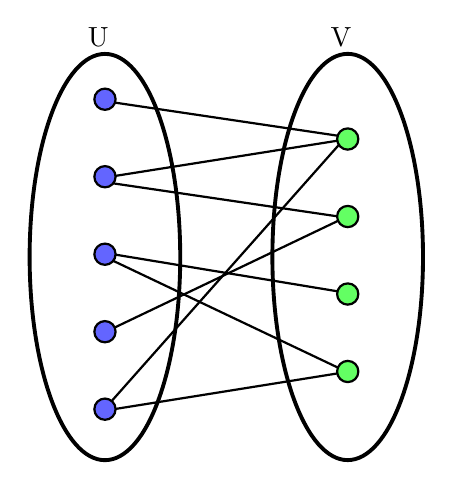
\begin{tikzpicture}[y=0.80pt, x=0.8pt,yscale=-0.5, xscale=0.5, inner sep=0pt, outer sep=0pt]
  \path[draw=black,line join=miter,line cap=butt,line width=0.800pt]
    (215.1625,381.6209) -- (421.2336,411.9255);
  \path[draw=black,line join=miter,line cap=butt,line width=0.800pt]
    (215.1625,586.4293) -- (428.3047,552.3367);
  \path[draw=black,line join=miter,line cap=butt,line width=0.800pt]
    (214.4049,445.5130) -- (428.5572,480.8684);
  \path[cm={{0.60283819,0.0,0.0,0.45550315,(91.98136,196.91071)}},draw=black,miter
    limit=4.00,line width=1.400pt] (308.5714,552.3622)arc(0.000:180.000:112.857140
    and 402.857)arc(-180.000:0.000:112.857140 and 402.857) -- cycle;
  \path[fill=black] (194.56386,258.44788) node[above right] (text3882) {U};
  \path[cm={{0.60283819,0.0,0.0,0.45550315,(311.29018,196.86231)}},draw=black,miter
    limit=4.00,line width=1.400pt] (308.5714,552.3622)arc(0.000:180.000:112.857140
    and 402.857)arc(-180.000:0.000:112.857140 and 402.857) -- cycle;
  \path[fill=black] (413.87268,258.39948) node[above right] (text3882-9) {V};
  \path[shift={(270.20979,112.61677)},draw=black,fill=c63ff63,miter
    limit=4.00,line width=0.800pt]
    (168.6955,299.2935)arc(0.000:180.000:9.596)arc(-180.000:0.000:9.596) -- cycle;
  \path[shift={(270.20979,252.61677)},draw=black,fill=c63ff63,miter
    limit=4.00,line width=0.800pt]
    (168.6955,299.2935)arc(0.000:180.000:9.596)arc(-180.000:0.000:9.596) -- cycle;
  \path[shift={(270.20979,182.61677)},draw=black,fill=c63ff63,miter
    limit=4.00,line width=0.800pt]
    (168.6955,299.2935)arc(0.000:180.000:9.596)arc(-180.000:0.000:9.596) -- cycle;
  \path[draw=black,line join=miter,line cap=butt,line width=0.800pt]
    (218.1929,308.8899) -- (422.2438,339.1945);
  \path[draw=black,line join=miter,line cap=butt,line width=0.800pt]
    (217.1828,375.5600) -- (421.2336,343.2351);
  \path[draw=black,line join=miter,line cap=butt,line width=0.800pt]
    (216.1726,451.3214) -- (420.2235,548.2961);
  \path[draw=black,line join=miter,line cap=butt,line width=0.800pt]
    (217.1828,512.9407) -- (420.2235,415.9661);
  \path[draw=black,line join=miter,line cap=butt,line width=0.800pt]
    (215.1625,579.6108) -- (421.2336,347.2757);
  \path[shift={(270.20979,42.616767)},draw=black,fill=c63ff63,miter
    limit=4.00,line width=0.800pt]
    (168.6955,299.2935)arc(0.000:180.000:9.596)arc(-180.000:0.000:9.596) -- cycle;
  \path[shift={(50.90097,6.665179)},draw=black,fill=c6365ff,miter limit=4.00,line
    width=0.800pt]
    (168.6955,299.2935)arc(0.000:180.000:9.596)arc(-180.000:0.000:9.596) -- cycle;
  \path[shift={(50.90097,76.665178)},draw=black,fill=c6365ff,miter limit=4.00,line
    width=0.800pt]
    (168.6955,299.2935)arc(0.000:180.000:9.596)arc(-180.000:0.000:9.596) -- cycle;
  \path[shift={(50.90097,146.66517)},draw=black,fill=c6365ff,miter limit=4.00,line
    width=0.800pt]
    (168.6955,299.2935)arc(0.000:180.000:9.596)arc(-180.000:0.000:9.596) -- cycle;
  \path[shift={(50.90097,216.66517)},draw=black,fill=c6365ff,miter limit=4.00,line
    width=0.800pt]
    (168.6955,299.2935)arc(0.000:180.000:9.596)arc(-180.000:0.000:9.596) -- cycle;
  \path[shift={(50.90097,286.66517)},draw=black,fill=c6365ff,miter limit=4.00,line
    width=0.800pt]
    (168.6955,299.2935)arc(0.000:180.000:9.596)arc(-180.000:0.000:9.596) -- cycle;

\end{tikzpicture}

  \end{center}
  \caption{A sample bipartite graph}
\end{wrapfigure}

A Bipartite graph is a graph which consists of two node sets. The nodes from
each set are only allowed to connect to nodes which are not a member of their
own set.

This model is able to generate realistic networks with low average path length,
high clustering coefficient and power-law distribution. The properties of the
network generated are dependent on the distribution of edges in the bipartite
graph.

The algorithm constructs a network in three simple steps:

\begin{enumerate}
   \item Generate a bipartite graph with two node sets e.g. set U and set V.
   \item Connect all nodes in U that are connected to the same node in V.
   \item Remove the nodes from set V from the graph.
\end{enumerate}

This procedure is implemented as follows: add the implementation ???

\subsection{Preferential Attachment with Clustering}

% FIXME
Preferential attachment and clustering are two distinct concepts which are used
in graph generation.

When using \emph{preferential attachment} we assign nodes in a network a preference
depending on their degree. Nodes with more edges, that is, which are more
connected will have a higher preference than nodes with less edges. The
preference ranges in $[0,1]$ and, assuming that no disjoint nodes exist and, is
\[ \frac{K_N}{Edges} \]
for a certain node $N$ with degree $N_K$, and $Edges$ being the total number of
edges.

\emph{Clustering} is a concept which determines how to connect a node $N$, once
a connection with at least one other node $N'$ has been established. This
procedure determines the intersection set of $N'$ with all its neighbours. Then
node $N$ is connected to all members of the intersection set.

The BA model has frequently been used to model real networks. A simple adaptation
of it increases the clustering whlist retaining the power-law degree distribution
of generated networks.

The bipartite nature of real networks can be interpreted as a tendency for cliques
to form in real networks. \emph{Cliques} are fully connected subsets of vertices of a
graph. Their presence greatly increases the clustering coefficient of a network.

In the original BA model, a new vertex is added to the network by preferential
attachment to a fixed number of vertices, whereas the algorithm described
 \emph{here} uses both concepts to generate networks with scale-free characteristics.
First, nodes are added to the network via the preferential attachment method.
Then, once attached they are connected to the rest of the network via the clustering procedure.
%% FIXME: i don't understand this phrase.

This is implemented as follows:

\begin{enumerate}
  \item
    Select a node by generating a random percentage with 2 decimal place
    precision.  The preferences of nodes are stored cumulatively. Therefore, the
    random number serves as an index with the node as the indexed element, which
    can be accessed using a binary search.

    %% FIXME: I don't understand this. What is Nodes? are you doing the binary
    %% search here? either way, it doesn't make sense
    \begin{algorithmic}
      \FOR{$l=1 \to N-1$}
        \STATE{$l \gets 2l$}
        \STATE{$i \gets 0$}
        \WHILE{$l \ge 0$}
	        \STATE $l \gets \frac{l}{2}$
	        \IF{$l+i \le N$}
		        \STATE pref $\gets$ real in  $[0,100]$
		        \IF{Comulative preference of $l$ $\leq$ pref}
		          \STATE $i \gets i+l$
		        \ENDIF
	        \ENDIF
	      \ENDWHILE
      \ENDFOR
      \RETURN Nodes[i]
    \end{algorithmic}

   \item
     Attach the node to the indexed element.

   \item
     Use the clustering procedure to determine other edges.

     \begin{algorithmic}
       \REQUIRE New Node $N_i$
       \REQUIRE Neighbour vector with all nodes neighbouring $N_i$
       \REQUIRE Edge count with amount of edges to be added
       \REQUIRE Used nodes vector
       \STATE length = neighbours.size

       \WHILE{There are edges to add $\land$ neighbour vector is not empty}
	       \STATE rand $\gets$ random integer $\bmod$ length
	       \STATE Node $R_i \gets$ neighbour[rand]
	       \IF{Edge creation between $N_i$ and $R_i$ was successful}
		       \STATE --edge count
		       \STATE add $R_i$ to used nodes vector
		       \STATE neighbour vector $\gets$ intersection(neighbour vector,neighbours($R_i$))
	       \ELSE
		       \STATE remove neighbours[rand]
	       \ENDIF
	       \STATE length $\gets$ neighbours.size()
       \ENDWHILE
     \end{algorithmic}

   \item
     If more edges are to be added, repeat the procedure.

   \item
     Recompute the preferences.
\end{enumerate}


\subsection{Real Small World Networks}
% FIXME
Finally, as Visigoth is supposed to help in analysing Small World
Networks, it can also fetch real world data from `live' social
networks Twitter and identi.ca.

\section{Statistics}


In addition to network generation Visigoth also calculates statistics about the
generated networks in real time. The statistics which are calculated are:


\begin{itemize}
	\item Average Degree
	\item Average Path Length
	\item Clustering Average
	\item Scale Free Exponent
	\item Clustering Coefficient
\end{itemize}

\subsection{Average Degree}
\[
\frac{2\sum_{i=1}^{\mathrm{max\ edges}} edges_i}{\sum_{j=1}^{\mathrm{max\
verticies}} vertecies_j}
\]

Implementation is trivial

\subsection{Average Path Length}
\[
\frac{\sum_{i,j}distance_\mathrm{shortest}(verticie_i,verticie_j)}{\sum
vertices^2 - \sum vertices}
\]

The first step in this algorithms is to calculate the path length from every
node to every node

\begin{algorithmic}
\FORALL{Nodes N}
	\STATE cumulativeLength $\gets$ lengthSum(N,visited,distance)
	\STATE \dots
\ENDFOR
\end{algorithmic}
Then divide the calculation by $N_i(N_i-1)$
\begin{algorithmic}
	\RETURN  $\frac{\mathrm{cummulativeLength}}{N(N-1)}$
\end{algorithmic}

Here \code{lengthSum} is a sub procedure which traverses the network in a
breadth-first manner and calculates the minimum distance to each node.
It then returns the sum of all distances

\begin{algorithmic}
\REQUIRE Starting node parent
\REQUIRE Queue of nodes adjecent to parent
\REQUIRE A vector of visited nodes called visited
\REQUIRE A distance vector
\WHILE{Queue is not empty}
	\STATE parent $\gets$ queue.dequeue()
	\STATE edges $\gets$ parent.edges()
	\FORALL{E in edges}
	\STATE Node n $\gets$ E.getDifferentFromParent()
		\IF{!visited.contain(n)}
			\STATE visited.insert(n)
			\STATE distance[n] $\gets$ distance.value(parent, 0) + 1
			\STATE queue.enqueue(n)
		\ENDIF
	\ENDFOR
	\STATE retLength += distance[parent]
\ENDWHILE

\RETURN retLength
\end{algorithmic}
\subsection{Clustering Coefficient}
\[
C_i = \frac{2|\{e_j,_k\}|}{k_i(k_i-1)}
\]
Where $k_i$ is the number of vertices immediately connected to $vertex_i$
\newline
The set ${e_j,_k}$ is set of all edges common to the neighbours of $vertex_i$\\

The first step is to calculate the intersection of the neighbours of the node wewant to calculate the statistic for and the neighbours of that node's neighbours
\begin{algorithmic}
\REQUIRE A node N
\REQUIRE An edge vector with edges connected to N
\REQUIRE A counter called intersection
\WHILE {!edges.empty()}
	\STATE Edge e $\gets$ edges.takeFirst()
	\STATE Vector nNeighbours = N.neighbours()
	\STATE Node $N_i \gets$ e.differentFrom(N)
	\STATE Vector otherNeighbours $\gets$  $N_i$.neighbours()
	\STATE  intersection += intersectionCount(nNeighbours, otherNeighbours);
\ENDWHILE
\end{algorithmic}
If the node's degree is greater than 1 we return the calculation.
\begin{algorithmic}
\REQUIRE k = N.degree()
\IF{k $>$ 1}
	\RETURN $\frac{2intersection}{k*(k-1)}$
\ELSE
	\RETURN 0
\ENDIF
\end{algorithmic}

\subsection{Clustering Average}
\[
C_\mathrm{avg} = \frac{1}{\mathrm{\sum vertecies}}\sum_{i=1}^{\mathrm{max\
vertecies}} C_i
\]
\begin{algorithmic}
\FORALL {Nodes N}
	\STATE clusterCumulative += clusteringCoeff(N)
\ENDFOR
\RETURN $\frac{clusterCumulative}{Node Cont}$
\end{algorithmic}

\subsection{Scale Free Exponent}

Before we are able to calculate any gradient Visigoth has to probe the network
and determine the degree distribution. Since we are dealing with exponential
growth, the algorithm takes the natural logarithm of both, the degree and its
frequency in the network, so that the gradient can be calculated as a straight
line.

\[
f(x) = ax^k \equiv ln(f(x)) = kln(a) + kln(x) \equiv y = mx + b
\]

\begin{algorithmic}
\REQUIRE maxDegree which holds the maximum degree of the network
\REQUIRE A vector to hold objects of type point
\FOR { $i = 0 \to maxDegree$}
	\STATE ++i
	\STATE count $\gets$ graph.nodesWithDegree(i)
	\STATE y = $\frac{count}{Total Nodes}$
	\IF { $y \ne 0$}
		\STATE  point p($ln(i+1)$,$ln(y)$)
		\STATE plot.add(p)
	\ENDIF
\ENDFOR
\end{algorithmic}

After the degree distribution has been recorded, the algorithm proceeds to
calculate the straight line gradient of the captured points.

\begin{algorithmic}
\REQUIRE A vector to hold objects of type point
\REQUIRE A counter c
\STATE $c = 0$
\FORALL {Point p in Plot}
	\IF { $c = 0$ }
		\STATE yPrev $\gets$ p.getY()
		\STATE  deltaX $\gets$ p.getX()
	\ELSE
		\STATE deltaX += p.getY() - yPref
		\STATE yPref $\gets$ p.getY()
		\STATE deltaX $\gets$ p.getX() - deltaX
	\ENDIF
		\STATE ++c
\ENDFOR
\RETURN $-1\frac{deltaY}{deltaX}$
\end{algorithmic}

The result is multiplied by -1 since the straight line gradient is downwards
sloping.



\section{Visigoth functionality}

% FIXME: Describe what we can do. Generate, set properties, save
%        screenshots, move nodes, fly in 3D, the kitchen sink.



\section{Visigoth technologies}

\subsection{Qt}

The UI toolkit, standard library replacement, and application
framework Visigoth uses is Qt\footnote{\url{http://qt.nokia.com/}}.

Visigoth relies heavily on some of Qt's features:
\begin{description}
\item [gui] Qt is famous for providing a cross-platform, high-level,
  UI toolkit that automatically uses the native drawing systems on
  each host platform. All of Visigoth's user visible interface was
  built using this framework. A more detailed explanation is included
  in Section \ref{gui};
\item [meta-objects] Qt supplements the venerable C
  pre-processor\footnote{\url{http://gcc.gnu.org/onlinedocs/cpp/}}
  with its own \buzz{meta-object
    compiler} \footnote{\url{http://developer.qt.nokia.com/doc/qt-4.8/moc.html}}.
  This preprocessor augments normal C++ objects with modern features
  such as introspection and \code{signal}s. We use introspection
  extensively in our tests; see Section \ref{tests}. We use
  \code{signal}s to decouple objects, which leads to a cleaner design
  and has the side-effect of simplifying writing test cases (mock and
  stub objects are not necessary anymore); for details, see Section
  \ref{interaction};
\item [xml] Like most modern frameworks, Qt provides an \buzz{XML}
  parsing
  library\footnote{\url{http://developer.qt.nokia.com/doc/qt-4.8/qtxml.html}}.
  In addition to a standard \buzz{SAX} parser, it exposes an extremely
  clean \buzz{HTML DOM}-like interface for manipulating \buzz{XML}
  documents. We use it in order to parse results from queries to
  online sources such as \href{http://twitter.com}{Twitter} and
  \href{http://identi.ca}{Identi.ca};
\item [containers] Qt provides a fully-featured library of containers
  similar to Java
  \buzz{collections} \footnote{\url{http://docs.oracle.com/javase/1.5.0/docs/api/java/util/package-summary.html}}
  and significantly more complete than the standard or SGI
  \buzz{STL}\footnote{\url{http://www.sgi.com/tech/stl/}}. The
  availability of these meant that advanced data-structures were one
  less concern to worry about during development;
\item [concurrency] Qt also provides high-level
  threading\footnote{\url{http://developer.qt.nokia.com/doc/qt-4.8/threads.html}}
  and
  concurrency\footnote{\url{http://developer.qt.nokia.com/doc/qt-4.8/threads-qtconcurrent.html}}
  APIs. Our experiments showed that separating the CPU-intensive
  computations (e.g. generating new networks, calculating layout
  positions) onto a separate thread could speed up certain operations
  by as much as a factor of $6$. The concurrency API, which provides
  functional programming style parallelized primitives
  (e.g. \code{map}, \code{filter}) could further improve performance.
  This is an area where further work could be done in Visigoth.
\end{description}

\subsubsection{Plugins}

Qt has a healthy plugin ecosystems, with a myriad of libraries
available to plug into the main framework. We make use of two of
these, namely
\buzz{QCA} \footnote{\url{http://delta.affinix.com/qca/}} and
\buzz{QOAuth} \footnote{\url{https://github.com/ayoy/qoauth/wiki}}.

\begin{description}
\item [QCA] The \buzz{Qt Cryptographic Architecture} includes many
  security providers for Qt application. We used the \buzz{OpenSSL}
  provider when establishing TLS-secured channels to the online
  sources (e.g. \href{http://twitter.com}{Twitter});
\item [QOAuth] This library is an implementation of the \buzz{OAuth
  2.0}\footnote{\url{http://oauth.net/}} secure API authorization
  standard (\buzz{OAuth} is becoming the de-facto authorization
  mechanism on the web); again, this was required in order to
  authenticate with the online sources.
\end{description}

\subsubsection{Cross-platform}

Thanks to Qt's cross-platform nature, in general, and to
\buzz{qmake} \footnote{\url{http://developer.qt.nokia.com/doc/qt-4.8/qmake-manual.html}},
in particular, Visigoth works on Windows, OSX and Linux with a minimum
of fuss on the development side.

\begin{description}
\item [qmake] Qt's build system, \buzz{qmake}, takes a high level
  project description and outputs platform-specific build files
  (\buzz{Makefile}s on Linux, \buzz{XCode} projects on OSX and
  \buzz{Visual Studio} projects on Windows). It also simplifies
  finding external libraries (by using its own mechanism on Linux,
  \buzz{pkg-config} on OSX and the registry on Windows).
\end{description}

The only tweaks necessary for Visigoth to build on each of the above
platforms are a few defines to deal with the misplaced \buzz{OpenGL}
headers on OSX and few conditionals in the project description to
handle the library finding on Windows.

The following screenshots show Visigoth working on the three
platforms.
%% FIXME: add screenshots

\subsubsection{Rapid prototyping}

One of lesser known advantages to using Qt we discovered is rapid
prototyping. Point in case, the original prototype for Visigoth took
two days to write. It included roughly half of the customer's
\emph{must-have} features, was cross-platform and was visually
impressive.

\subsection{OpenGL}
\label{opengl}

After being left unsatisfied with the performance achieved with a
screen renderer using Qt graphics primitives, we looked for a `bare-metal'
graphics output solution in order to eliminate the graphics bottleneck.
Thanks to OpenGL\footnote{OpenGL documentation:
https://www.opengl.org/documentation/},
we can now draw even large graphs very quickly,
no matter whether in 2D or in 3D.

OpenGL itself is a graphics drawing interface commonly used to
leverage hardware acceleration for common operations, such as vector
transformations necessary to compute 3D graphics. Every modern
operating system uses it to animate its user interface smoothly,
and games and professional CAD (Computer Assisted Design) applications
have long used it for real-time 3D graphics interaction.

Not only are we leveraging this power to speed up our graph
visualiser, but this may also allow for ports to other
platforms in the future. Thanks to the Qt/OpenGL base, Visigoth
could theoretically be compiled for mobile phones and slates
with minimal porting effort.

OpenGL made several extensions possible, as outlined in the following
subsections.

\subsubsection{3D graphs and camera}
OpenGL provides only the very fundamental drawing primitives like
lines and points - however, it includes hardware acceleration for
vector transformation. This allows the implementation of a virtual
3D space through which a `camera' can move. As even this is actually
a composite functionality, we wrote a helper code library (glAncillary)
to provide us with easy camera transformation functions. They are
used whenever the user decides to move around the graph, i.e. to
pan or tilt.

\subsubsection{Selection}
The OpenGL interface also eases object selection: Since it is
responsible for the depth transformations when drawing the graphics,
it can also perform the inverse of these transformations from any
given point on the drawing surface, finding the original point
in space. In this case we check the position the mouse pointer is at
and find the object selected by the user. This is fundamental in
allowing us to move nodes around and selecting them for statistical
analysis.

\subsection{C++}

Visigoth, ignoring the XML files describing the interface, is entirely
written in \buzz{C++}. Initially, while being conscious of its disadvantages,
we made this decision for one reason: \buzz{Qt}. As described in the previous
paragraph, the library by TrollTech is so convenient that alone
justifies the use of C++ instead of another safer language.

All in all, we think it was the right decision. The appreciation of
C++ varies in our team, but looking back we are confident that C++ was
one of the best choices considering the nature of the application we
have been developing.

The main advantages were:

\begin{description}

\item [Availability of tools and library] As mentioned, \buzz{Qt} alone
  was a deal sealer, but the fact that we were able to access OpenGL
  `natively' (in a Qt widget) was also a big advantage. While interfaces
  to both libraries exist in other languages as well, we felt that
  sticking to Qt's `native' C++ environment would be the most stable
  solution and that the foreign language bindings would have degraded
  performance.

\item [Performance] We did not consider this factor at the beginning,
  but a few weeks into the project we started hitting various
  bottlenecks. We can only speculate about actual performance gains,
  but the fact that we were using
  C++ allowed us to fine-tune the application (specifically on the
  memory management side) in a way that we would not be able to do
  with managed languages. Furthermore, having an optimising compiler
  instead of an interpreter or JIT (as it would have been the case
  using a language like Python or Ruby) aided performance as well.

\item [Abstraction] The previous two points (especially the second)
  are partly shared by C++ with its predecessor, C. However, the
  possibility to structure our code into classes facilitates greatly
  structuring a medium sized application like Visigoth, especially
  considering that we had to coordinate five people working together.
  For example, there is a common \code{Algorithm} interface which all
  graph generation algorithms have to implement. They can then
  be plugged into the main widget at will: this kind of operation
  would have been much more laborious and less type-safe in C.

\end{description}

However, C++ also has its downsides:

\begin{description}

\item [Unmanaged memory] This is by far C++'s most ``dangerous''
  feature (or better, lack of feature). While enabling greater control
  and thus greater performance, it requires a much more attentive
  analysis of the code. This is in a way a good thing, since it forces
  the programmer to reason more about what the code is doing; but it
  also paves the way to a nasty class of bugs and memory leaks that
  more than once took hours (in one case days) to track down. This is
  a somewhat controversial subject in our team as well as the broader
  programming community and our opinions differ on how much better a
  garbage collected language would have been when considering the loss in
  performance. C++ also has the characteristic (required by its
  unmanaged nature) of allowing objects to be used in the heap through
  pointers and on the stack as values, which slows down compilation
  considerably - when changing a header file, all code that uses
  that object as a value has to be recompiled. Moreover, C++ allows two
  kinds of references: immutable references and C-style pointers, the
  former with
  a rather confusing syntax - references are indistinguishable from
  values when used. All these factors generate much confusion which is
  absent in most modern O-O languages.

\item [Language bloat] C++ is a very broad language with a number of
  esoteric language features. Notable examples are templates, operator
  overloading and ``friend'' attributes. Some of them are very
  useful and never harmful, e.g. the \code{const} keyword is a
  great mechanism to mark immutability at type level. However, some
  of them can and have been misused\footnote{For an hilarious example,
    see
    \url{http://weegen.home.xs4all.nl/eelis/analogliterals.xhtml}},
  and as a consequence ``when you're programming C++ no one can ever
  agree on which ten percent of the language is safe to use'' (Jamie
  Zawinski). This kind of ``programming language discipline'' is
  required when working on a C++ project and we had our fair share
  of arguments on which subset of the language is safe to use;
  nevertheless we think we have managed to keep the code clean to
  high standards in the C++ world.

\end{description}

This is of course only a very brief analysis of C++, but it does
highlight the points that we felt the most while developing Visigoth.




\section{Engineering Visigoth}
%% This section corresponds to C in the requirements

We encountered a number of difficulties whilst building Visigoth,
which we overcame by dividing the application into mostly-independent
components. The following sections provide overviews and short
descriptions for each component.

\subsection{GUI}
\label{gui}

Since Visigoth is an end-user-oriented application, the GUI is, by
far, the most important component. Luckily, the user work-flows we
considered contain very few steps (hence, there is little need for
``Wizards'' or nested-design).

As shown in Figure \ref{fig:gui-sketch}, the Visigoth UI is
\emph{flat}. All relevant options and displays are presented to the
user in a single encompassing interface. Relevancy is determined by
context; for instance, the generation parameters (Figure
\ref{fig:gui-sketch}.3) vary depending on the algorithm selected (in
Figure \ref{fig:gui-sketch}.1).

\begin{figure}[h]
  \centering
  
\definecolor{c2b1100}{RGB}{43,17,0}

\begin{tikzpicture}[y=0.80pt, x=0.8pt,yscale=-1, inner sep=0pt, outer sep=0pt]
\begin{scope}[shift={(-235.60247,-129.32997)}]
    \path[draw=c2b1100,line join=miter,line cap=butt,miter limit=4.00,line
      width=0.800pt,rounded corners=0.0000cm] (246.1028,139.8300) rectangle
      (545.7283,376.0971);
    \path[draw=c2b1100,line join=miter,line cap=butt,miter limit=4.00,line
      width=0.800pt,rounded corners=0.0000cm] (455.1049,187.9840) rectangle
      (540.7122,212.7299);
    \path[fill=black] (495.20386,204.3949) node[above right] (text2995) {1       };
    \path[cm={{0.46816479,0.0,0.0,0.46816479,(423.67103,-163.24222)}},draw=c2b1100,line
      join=miter,line cap=butt,miter limit=4.00,line width=1.709pt]
      (174.2857,776.6479) .. controls (174.2857,785.3266) and (167.2502,792.3622) ..
      (158.5714,792.3622) .. controls (149.8927,792.3622) and (142.8571,785.3266) ..
      (142.8571,776.6479) .. controls (142.8571,767.9691) and (149.8927,760.9336) ..
      (158.5714,760.9336) .. controls (167.2502,760.9336) and (174.2857,767.9691) ..
      (174.2857,776.6479) -- cycle;
    \path[draw=c2b1100,line join=miter,line cap=butt,miter limit=4.00,line
      width=0.800pt,rounded corners=0.0000cm] (455.1021,220.4184) rectangle
      (540.7150,278.6103);
    \path[fill=black] (494.91574,253.55225) node[above right] (text3772) {2       };
    \path[cm={{0.46816479,0.0,0.0,0.46816479,(423.67096,-114.08487)}},draw=c2b1100,line
      join=miter,line cap=butt,miter limit=4.00,line width=1.709pt]
      (174.2857,776.6479) .. controls (174.2857,785.3266) and (167.2502,792.3622) ..
      (158.5714,792.3622) .. controls (149.8927,792.3622) and (142.8571,785.3266) ..
      (142.8571,776.6479) .. controls (142.8571,767.9691) and (149.8927,760.9336) ..
      (158.5714,760.9336) .. controls (167.2502,760.9336) and (174.2857,767.9691) ..
      (174.2857,776.6479) -- cycle;
    \path[draw=c2b1100,line join=miter,line cap=butt,miter limit=4.00,line
      width=0.800pt,rounded corners=0.0000cm] (454.4333,286.2957) rectangle
      (540.0462,353.8509);
    \path[fill=black] (494.13446,324.03989) node[above right] (text3778) {3       };
    \path[cm={{0.46816479,0.0,0.0,0.46816479,(423.00216,-43.52589)}},draw=c2b1100,line
      join=miter,line cap=butt,miter limit=4.00,line width=1.709pt]
      (174.2857,776.6479) .. controls (174.2857,785.3266) and (167.2502,792.3622) ..
      (158.5714,792.3622) .. controls (149.8927,792.3622) and (142.8571,785.3266) ..
      (142.8571,776.6479) .. controls (142.8571,767.9691) and (149.8927,760.9336) ..
      (158.5714,760.9336) .. controls (167.2502,760.9336) and (174.2857,767.9691) ..
      (174.2857,776.6479) -- cycle;
    \path[draw=c2b1100,line join=miter,line cap=butt,miter limit=4.00,line
      width=0.800pt,rounded corners=0.0000cm] (251.1188,187.9841) rectangle
      (449.0856,353.8482);
    \path[fill=black] (347.17804,274.93759) node[above right] (text3784) {4       };
    \path[cm={{0.46816479,0.0,0.0,0.46816479,(275.86469,-92.683076)}},draw=c2b1100,line
      join=miter,line cap=butt,miter limit=4.00,line width=1.709pt]
      (174.2857,776.6479) .. controls (174.2857,785.3266) and (167.2502,792.3622) ..
      (158.5714,792.3622) .. controls (149.8927,792.3622) and (142.8571,785.3266) ..
      (142.8571,776.6479) .. controls (142.8571,767.9691) and (149.8927,760.9336) ..
      (158.5714,760.9336) .. controls (167.2502,760.9336) and (174.2857,767.9691) ..
      (174.2857,776.6479) -- cycle;
    \path[fill=black] (392.78284,152.82375) node[above right] (text3790) {5       };
    \path[cm={{0.46816479,0.0,0.0,0.46816479,(321.67797,-214.67346)}},draw=c2b1100,line
      join=miter,line cap=butt,miter limit=4.00,line width=1.709pt]
      (174.2857,776.6479) .. controls (174.2857,785.3266) and (167.2502,792.3622) ..
      (158.5714,792.3622) .. controls (149.8927,792.3622) and (142.8571,785.3266) ..
      (142.8571,776.6479) .. controls (142.8571,767.9691) and (149.8927,760.9336) ..
      (158.5714,760.9336) .. controls (167.2502,760.9336) and (174.2857,767.9691) ..
      (174.2857,776.6479) -- cycle;
    \path[fill=black] (392.83771,171.88919) node[above right] (text3796) {6       };
    \path[cm={{0.46816479,0.0,0.0,0.46816479,(321.67797,-195.67934)}},draw=c2b1100,line
      join=miter,line cap=butt,miter limit=4.00,line width=1.709pt]
      (174.2857,776.6479) .. controls (174.2857,785.3266) and (167.2502,792.3622) ..
      (158.5714,792.3622) .. controls (149.8927,792.3622) and (142.8571,785.3266) ..
      (142.8571,776.6479) .. controls (142.8571,767.9691) and (149.8927,760.9336) ..
      (158.5714,760.9336) .. controls (167.2502,760.9336) and (174.2857,767.9691) ..
      (174.2857,776.6479) -- cycle;
    \path[fill=black] (392.78012,371.19363) node[above right] (text3802) {7       };
    \path[cm={{0.46816479,0.0,0.0,0.46816479,(321.67797,3.6250996)}},draw=c2b1100,line
      join=miter,line cap=butt,miter limit=4.00,line width=1.709pt]
      (174.2857,776.6479) .. controls (174.2857,785.3266) and (167.2502,792.3622) ..
      (158.5714,792.3622) .. controls (149.8927,792.3622) and (142.8571,785.3266) ..
      (142.8571,776.6479) .. controls (142.8571,767.9691) and (149.8927,760.9336) ..
      (158.5714,760.9336) .. controls (167.2502,760.9336) and (174.2857,767.9691) ..
      (174.2857,776.6479) -- cycle;
    \path[draw=black,line join=miter,line cap=butt,miter limit=4.00,line
      width=0.800pt] (246.1025,158.2890) -- (545.3547,158.2890);
    \path[draw=black,line join=miter,line cap=butt,miter limit=4.00,line
      width=0.800pt] (246.1025,177.9520) -- (545.3547,177.9520);
    \path[draw=black,line join=miter,line cap=butt,miter limit=4.00,line
      width=0.800pt] (246.1025,357.7272) -- (545.3547,357.7272);
\end{scope}

\end{tikzpicture}

  \caption{UI wire-frame sketch: 1. Generation algorithm chooser;
    2. Statistics; 3. Generation parameters; 4. Graph display; 5. Main
    menu; 6. Quick actions; 7. Status bar}
  \label{fig:gui-sketch}
\end{figure}

\noindent The most general user work-flow is as follows:
\begin{description}
  \setlength{\itemindent}{\parindent}
  \item [Figure \ref{fig:gui-sketch}.1] User selects a generation
    algorithm;
  \item [Figure \ref{fig:gui-sketch}.2] User checks whether the graph
    has the properties desired and
  \item [Figure \ref{fig:gui-sketch}.3] tweaks the parameters;
  \item [Figure \ref{fig:gui-sketch}.4] User checks the generated
    graph and, if necessary, manually adjusts its layout;
  \item [Figure \ref{fig:gui-sketch}.5, 6] User decides to save the
    generated graph to a file or to an image.
\end{description}

\subsection{Components}
\label{components}
%% This is an overview of the classes (including a class diagram).

The \emph{[mostly]} independent components of Visigoth are:
\begin{description}
  \item [tests] The test system is heavily oriented towards
    functionality testing, checking that user actions cause the
    expected behaviour. For more details on the testing methodology,
    see Section \ref{tests};

  \item [GUI] The GUI is the only user-visible component. It was
    relies heavily on Qt's widget library and OpenGL. A brief
    description of the UI is provided in Section \ref{gui}, and a
    brief overview of the issues surrounding the 3D renderer can be
    found in Section \ref{opengl};

  \item [GraphScene] We took an \buzz{Model-View-Controller} approach
    in Visigoth's design. Whist the GUI system is the View, the
    \code{GraphScene} is the model and encapsulates the
    controller. For a brief description on how it is used, see Section
    \ref{interaction};

  \item [Algorithm] The last component of Visigoth are the
    algorithms. These were described in Section
    \ref{smallworldnetworks}. All the individual algorithms implement
    the \code{Algorithm} interface, which allows them to be easily
    plugged into the \code{GraphScene}.
\end{description}

A bare-bones class diagram of the above components is include in
Figure \ref{fig:classes}. Since the internal workings of the classes
are unlikely to be of interest to the reader and to highlight the
relationships between components, we only include inheritance and
usages.

\begin{figure}[ht]
  \centering
  
\definecolor{c2b1100}{RGB}{43,17,0}

\begin{tikzpicture}[y=0.80pt, x=0.8pt,yscale=-1, inner sep=0pt, outer sep=0pt]
\begin{scope}[shift={(-174.90031,-221.35276)}]
    \path[cm={{1.0,0.0,-0.25881906,0.96592582,(0.0,0.0)}},draw=c2b1100,line
      join=miter,line cap=butt,miter limit=4.00,line width=0.814pt,rounded
      corners=0.0000cm] (519.1957,689.8035) rectangle (588.3925,706.1153);
    \path[cm={{1.0,0.0,-0.26794921,1.0,(0.0,0.0)}},fill=black] (527.67328,682.25549)
      node[above right] (text2987) {Algorithm     };
    \path[fill=black] (496.41861,726.57574) node[above right] (text3043) {Twitter
      };
    \path[draw=c2b1100,line join=miter,line cap=butt,miter limit=4.00,line
      width=0.800pt,rounded corners=0.0000cm] (492.9985,713.3670) rectangle
      (540.3671,729.1670);
    \path[fill=black] (211.3568,728.34882) node[above right] (text3007) {ErdosRenyi
      };
    \path[draw=c2b1100,line join=miter,line cap=butt,miter limit=4.00,line
      width=0.800pt,rounded corners=0.0000cm] (205.9307,713.3976) rectangle
      (280.2136,729.1363);
    \path[fill=black] (233.92371,751.40686) node[above right] (text2991)
      {BarabasiAlbert       };
    \path[draw=c2b1100,line join=miter,line cap=butt,miter limit=4.00,line
      width=0.800pt,rounded corners=0.0000cm] (227.7710,738.1706) rectangle
      (321.1261,754.0257);
    \path[fill=black] (434.84686,752.258) node[above right] (text3055)
      {WattsStrogatz       };
    \path[draw=c2b1100,line join=miter,line cap=butt,miter limit=4.00,line
      width=0.800pt,rounded corners=0.0000cm] (427.4141,738.1981) rectangle
      (518.5268,753.9981);
    \path[fill=black] (304.90619,774.91241) node[above right] (text2999) {Bipartite
      };
    \path[draw=c2b1100,line join=miter,line cap=butt,miter limit=4.00,line
      width=0.800pt,rounded corners=0.0000cm] (298.3260,760.8566) rectangle
      (356.7958,776.6545);
    \path[fill=black] (380.16458,774.13904) node[above right] (text3027)
      {Preferential       };
    \path[draw=c2b1100,line join=miter,line cap=butt,miter limit=4.00,line
      width=0.800pt,rounded corners=0.0000cm] (375.0404,760.8328) rectangle
      (447.9719,776.6782);
  \path[draw=c2b1100,line join=miter,line cap=butt,miter limit=4.00,line
    width=0.800pt,rounded corners=0.0000cm] (185.4003,637.4907) rectangle
    (560.8975,787.1140);
  \path[fill=black] (344.63321,651.64423) node[above right] (text8048) {Algorithm
    };
    \path[fill=black] (338.94666,553.91602) node[above right] (text3015) {GraphScene
      };
    \path[draw=c2b1100,line join=miter,line cap=butt,miter limit=4.00,line
      width=0.800pt,rounded corners=0.0000cm] (334.7563,539.7668) rectangle
      (412.0519,555.6020);
    \path[fill=black] (445.23074,604.19696) node[above right] (text3003) {Edge
      };
    \path[draw=c2b1100,line join=miter,line cap=butt,miter limit=4.00,line
      width=0.800pt,rounded corners=0.0000cm] (434.5910,589.2089) rectangle
      (484.8885,605.0215);
    \path[fill=black] (370.77048,602.49573) node[above right] (text3035) {Statistics
      };
    \path[draw=c2b1100,line join=miter,line cap=butt,miter limit=4.00,line
      width=0.800pt,rounded corners=0.0000cm] (367.9417,589.1925) rectangle
      (422.6464,605.0379);
    \path[fill=black] (500.56403,602.42395) node[above right] (text3023) {Node
      };
    \path[draw=c2b1100,line join=miter,line cap=butt,miter limit=4.00,line
      width=0.800pt,rounded corners=0.0000cm] (496.8331,589.2151) rectangle
      (533.9948,605.0152);
    \path[fill=black] (295.83789,604.22595) node[above right] (text3031) {QuadTree
      };
    \path[draw=c2b1100,line join=miter,line cap=butt,miter limit=4.00,line
      width=0.800pt,rounded corners=0.0000cm] (290.3776,589.2031) rectangle
      (355.9972,605.0273);
  \path[fill=black] (337.25412,525.9975) node[above right] (text8260) {GraphScene
    };
  \path[draw=c2b1100,line join=miter,line cap=butt,miter limit=4.00,line
    width=0.800pt,rounded corners=0.0000cm] (185.4003,512.3205) rectangle
    (561.4079,617.3446);
    \path[fill=black] (217.17059,603.20026) node[above right] (text8178) {Algorithm
      };
    \path[draw=c2b1100,line join=miter,line cap=butt,miter limit=4.00,line
      width=0.800pt,rounded corners=0.0000cm] (212.8134,589.2031) rectangle
      (278.4330,605.0273);
    \path[draw=c2b1100,line join=miter,line cap=butt,miter limit=4.00,line
      width=0.725pt] (209.3740,589.9500) .. controls (209.3740,596.9025) and
      (209.3740,603.8551) .. (209.3740,610.8077) .. controls (233.5418,610.8077) and
      (257.7095,610.8077) .. (281.8773,610.8077) .. controls (281.8773,601.6821) and
      (281.8773,592.5566) .. (281.8773,583.4310) .. controls (257.7096,583.4310) and
      (233.5418,583.4310) .. (209.3740,583.4310) .. controls (209.3740,585.6040) and
      (209.3740,587.7770) .. (209.3740,589.9500) -- cycle;
    \path[fill=black] (349.01846,364.20969) node[above right] (text3019) {MainWindow
      };
    \path[draw=c2b1100,line join=miter,line cap=butt,miter limit=4.00,line
      width=0.800pt,rounded corners=0.0000cm] (341.0906,350.1661) rectangle
      (427.8468,367.6358);
    \path[fill=black] (344.43729,334.3941) node[above right] (text3993) {QMainWindow
      };
    \path[draw=c2b1100,line join=miter,line cap=butt,miter limit=4.00,line
      width=0.800pt,rounded corners=0.0000cm] (334.8936,319.6544) rectangle
      (434.0439,336.9058);
    \path[fill=black] (282.29581,441.0975) node[above right] (text3011)
      {GLGraphWidget       };
    \path[draw=c2b1100,line join=miter,line cap=butt,miter limit=4.00,line
      width=0.800pt,rounded corners=0.0000cm] (272.9869,426.2390) rectangle
      (380.6145,443.6365);
    \path[fill=black] (266.82867,478.84314) node[above right] (text3047) {VCubeF
      };
    \path[draw=c2b1100,line join=miter,line cap=butt,miter limit=4.00,line
      width=0.800pt,rounded corners=0.0000cm] (258.3968,465.5352) rectangle
      (319.6728,481.3902);
    \path[fill=black] (343.45309,478.77136) node[above right] (text3051) {VPointF
      };
  \path[draw=c2b1100,line join=miter,line cap=butt,miter limit=4.00,line
    width=0.800pt,rounded corners=0.0000cm] (334.7740,465.5933) rectangle
    (395.2047,481.3320);
    \path[fill=black] (244.02667,396.08804) node[above right] (text4009) {QGLWidget
      };
    \path[draw=c2b1100,line join=miter,line cap=butt,miter limit=4.00,line
      width=0.800pt,rounded corners=0.0000cm] (236.7780,381.0354) rectangle
      (314.7539,396.8218);
    \path[fill=black] (431.61746,441.0975) node[above right] (text8334) {GraphScene
      };
    \path[draw=c2b1100,line join=miter,line cap=butt,miter limit=4.00,line
      width=0.800pt,rounded corners=0.0000cm] (426.5960,426.9728) rectangle
      (505.5539,442.7592);
    \path[draw=c2b1100,line join=miter,line cap=butt,miter limit=4.00,line
      width=0.762pt] (421.5986,427.3390) .. controls (421.5986,434.6404) and
      (421.5986,441.9417) .. (421.5986,449.2431) .. controls (451.2499,449.2431) and
      (480.9013,449.2431) .. (510.5526,449.2431) .. controls (510.5526,439.6566) and
      (510.5526,430.0700) .. (510.5526,420.4835) .. controls (480.9013,420.4835) and
      (451.2499,420.4835) .. (421.5986,420.4835) .. controls (421.5986,422.7687) and
      (421.5986,425.0538) .. (421.5986,427.3390) -- cycle;
  \path[draw=c2b1100,line join=miter,line cap=butt,miter limit=4.00,line
    width=0.800pt,rounded corners=0.0000cm] (185.4003,293.6357) rectangle
    (561.9182,492.1744);
  \path[fill=black] (362.87619,305.86453) node[above right] (text9031) {GUI     };
  \path[draw=c2b1100,dash pattern=on 2.40pt off 0.80pt,line join=miter,line
    cap=butt,miter limit=4.00,line width=0.800pt,rounded corners=0.0000cm]
    (211.7161,373.8237) rectangle (402.9694,487.7619);
  \begin{scope}[cm={{0.0,-1.0,1.0,0.0,(0.0,0.0)}},fill=black]
    \path[fill] (-461.3479,205.3749) -- (-460.2714,205.2313) .. controls
      (-460.1478,205.8414) and (-459.9385,206.2819) .. (-459.6434,206.5531) ..
      controls (-459.3444,206.8202) and (-458.9816,206.9538) .. (-458.5550,206.9538)
      .. controls (-458.0486,206.9538) and (-457.6220,206.7783) ..
      (-457.2751,206.4275) .. controls (-456.9242,206.0766) and (-456.7488,205.6420)
      .. (-456.7488,205.1237) .. controls (-456.7488,204.6293) and
      (-456.9103,204.2226) .. (-457.2332,203.9037) .. controls (-457.5562,203.5807)
      and (-457.9669,203.4192) .. (-458.4652,203.4192) .. controls
      (-458.6686,203.4192) and (-458.9218,203.4591) .. (-459.2248,203.5388) --
      (-459.1052,202.5939) .. controls (-459.0334,202.6019) and (-458.9756,202.6059)
      .. (-458.9317,202.6059) .. controls (-458.4732,202.6059) and
      (-458.0605,202.4863) .. (-457.6937,202.2471) .. controls (-457.3269,202.0078)
      and (-457.1435,201.6390) .. (-457.1435,201.1406) .. controls
      (-457.1435,200.7459) and (-457.2771,200.4190) .. (-457.5442,200.1598) ..
      controls (-457.8114,199.9007) and (-458.1562,199.7711) .. (-458.5789,199.7711)
      .. controls (-458.9975,199.7711) and (-459.3464,199.9027) ..
      (-459.6255,200.1658) .. controls (-459.9046,200.4289) and (-460.0840,200.8237)
      .. (-460.1637,201.3500) -- (-461.2403,201.1586) .. controls
      (-461.1087,200.4369) and (-460.8096,199.8787) .. (-460.3432,199.4840) ..
      controls (-459.8767,199.0853) and (-459.2965,198.8859) .. (-458.6028,198.8859)
      .. controls (-458.1243,198.8859) and (-457.6838,198.9896) ..
      (-457.2811,199.1969) .. controls (-456.8784,199.4003) and (-456.5714,199.6794)
      .. (-456.3600,200.0342) .. controls (-456.1448,200.3891) and
      (-456.0371,200.7659) .. (-456.0371,201.1646) .. controls (-456.0371,201.5433)
      and (-456.1388,201.8882) .. (-456.3421,202.1992) .. controls
      (-456.5455,202.5102) and (-456.8465,202.7574) .. (-457.2452,202.9408) ..
      controls (-456.7269,203.0604) and (-456.3242,203.3096) .. (-456.0371,203.6884)
      .. controls (-455.7500,204.0632) and (-455.6065,204.5337) ..
      (-455.6065,205.0998) .. controls (-455.6065,205.8653) and (-455.8856,206.5152)
      .. (-456.4438,207.0495) .. controls (-457.0020,207.5798) and
      (-457.7077,207.8449) .. (-458.5609,207.8449) .. controls (-459.3304,207.8449)
      and (-459.9704,207.6157) .. (-460.4807,207.1572) .. controls
      (-460.9871,206.6986) and (-461.2761,206.1046) .. (-461.3479,205.3749);
    \path[fill] (-454.0994,207.6894) -- (-454.0994,198.9218) -- (-451.0792,198.9218)
      .. controls (-450.3974,198.9218) and (-449.8770,198.9637) ..
      (-449.5182,199.0474) .. controls (-449.0158,199.1630) and (-448.5872,199.3723)
      .. (-448.2324,199.6753) .. controls (-447.7699,200.0661) and
      (-447.4250,200.5665) .. (-447.1977,201.1765) .. controls (-446.9665,201.7825)
      and (-446.8508,202.4763) .. (-446.8508,203.2577) .. controls
      (-446.8508,203.9236) and (-446.9286,204.5137) .. (-447.0841,205.0280) ..
      controls (-447.2396,205.5423) and (-447.4389,205.9690) .. (-447.6821,206.3079)
      .. controls (-447.9254,206.6428) and (-448.1925,206.9079) ..
      (-448.4835,207.1033) .. controls (-448.7706,207.2947) and (-449.1195,207.4402)
      .. (-449.5302,207.5399) .. controls (-449.9368,207.6396) and
      (-450.4053,207.6894) .. (-450.9356,207.6894) --
      (-454.0994,207.6894)(-452.9391,206.6547) -- (-451.0672,206.6547) .. controls
      (-450.4891,206.6547) and (-450.0365,206.6009) .. (-449.7096,206.4933) ..
      controls (-449.3787,206.3856) and (-449.1155,206.2341) .. (-448.9201,206.0387)
      .. controls (-448.6450,205.7636) and (-448.4317,205.3948) ..
      (-448.2802,204.9323) .. controls (-448.1247,204.4658) and (-448.0470,203.9017)
      .. (-448.0470,203.2398) .. controls (-448.0470,202.3228) and
      (-448.1985,201.6191) .. (-448.5015,201.1286) .. controls (-448.8005,200.6342)
      and (-449.1653,200.3033) .. (-449.5959,200.1358) .. controls
      (-449.9069,200.0162) and (-450.4073,199.9564) .. (-451.0971,199.9564) --
      (-452.9391,199.9564) -- (-452.9391,206.6547);
    \path[fill] (-441.8570,207.6894) -- (-441.8570,198.9218) -- (-437.9696,198.9218)
      .. controls (-437.1881,198.9218) and (-436.5940,199.0015) ..
      (-436.1873,199.1610) .. controls (-435.7807,199.3165) and (-435.4557,199.5936)
      .. (-435.2125,199.9923) .. controls (-434.9693,200.3910) and
      (-434.8477,200.8316) .. (-434.8477,201.3140) .. controls (-434.8477,201.9360)
      and (-435.0490,202.4603) .. (-435.4517,202.8869) .. controls
      (-435.8544,203.3136) and (-436.4764,203.5847) .. (-437.3177,203.7003) ..
      controls (-437.0107,203.8478) and (-436.7774,203.9934) .. (-436.6180,204.1369)
      .. controls (-436.2791,204.4479) and (-435.9581,204.8366) ..
      (-435.6551,205.3031) -- (-434.1300,207.6894) -- (-435.5893,207.6894) --
      (-436.7495,205.8653) .. controls (-437.0884,205.3390) and (-437.3675,204.9363)
      .. (-437.5868,204.6572) .. controls (-437.8061,204.3781) and
      (-438.0035,204.1827) .. (-438.1789,204.0711) .. controls (-438.3504,203.9595)
      and (-438.5258,203.8817) .. (-438.7052,203.8379) .. controls
      (-438.8368,203.8100) and (-439.0521,203.7960) .. (-439.3511,203.7960) --
      (-440.6968,203.7960) -- (-440.6968,207.6894) --
      (-441.8570,207.6894)(-440.6968,202.7912) -- (-438.2028,202.7912) .. controls
      (-437.6725,202.7912) and (-437.2579,202.7374) .. (-436.9589,202.6297) ..
      controls (-436.6598,202.5181) and (-436.4326,202.3427) .. (-436.2771,202.1034)
      .. controls (-436.1216,201.8602) and (-436.0438,201.5971) ..
      (-436.0438,201.3140) .. controls (-436.0438,200.8993) and (-436.1953,200.5584)
      .. (-436.4983,200.2913) .. controls (-436.7974,200.0242) and
      (-437.2718,199.8906) .. (-437.9217,199.8906) -- (-440.6968,199.8906) --
      (-440.6968,202.7912);
    \path[fill] (-428.8132,205.6440) -- (-427.7008,205.7816) .. controls
      (-427.8763,206.4315) and (-428.2012,206.9358) .. (-428.6757,207.2947) ..
      controls (-429.1501,207.6535) and (-429.7562,207.8329) .. (-430.4938,207.8329)
      .. controls (-431.4228,207.8329) and (-432.1604,207.5479) ..
      (-432.7066,206.9777) .. controls (-433.2489,206.4036) and (-433.5200,205.6002)
      .. (-433.5200,204.5675) .. controls (-433.5200,203.4990) and
      (-433.2449,202.6697) .. (-432.6947,202.0796) .. controls (-432.1444,201.4895)
      and (-431.4308,201.1944) .. (-430.5536,201.1944) .. controls
      (-429.7043,201.1944) and (-429.0106,201.4835) .. (-428.4723,202.0616) ..
      controls (-427.9341,202.6397) and (-427.6650,203.4531) .. (-427.6649,204.5017)
      .. controls (-427.6650,204.5655) and (-427.6669,204.6612) ..
      (-427.6709,204.7888) -- (-432.4076,204.7888) .. controls (-432.3677,205.4865)
      and (-432.1704,206.0208) .. (-431.8155,206.3916) .. controls
      (-431.4607,206.7624) and (-431.0181,206.9478) .. (-430.4878,206.9478) ..
      controls (-430.0931,206.9478) and (-429.7562,206.8441) .. (-429.4771,206.6368)
      .. controls (-429.1980,206.4295) and (-428.9767,206.0985) ..
      (-428.8132,205.6440)(-432.3478,203.9036) -- (-428.8013,203.9036) .. controls
      (-428.8491,203.3694) and (-428.9847,202.9687) .. (-429.2080,202.7015) ..
      controls (-429.5509,202.2869) and (-429.9954,202.0796) .. (-430.5417,202.0795)
      .. controls (-431.0360,202.0796) and (-431.4527,202.2450) ..
      (-431.7916,202.5759) .. controls (-432.1265,202.9069) and (-432.3119,203.3494)
      .. (-432.3478,203.9036);
    \path[fill] (-426.3432,207.6894) -- (-426.3432,201.3380) -- (-425.3743,201.3380)
      -- (-425.3743,202.2410) .. controls (-424.9079,201.5433) and
      (-424.2340,201.1944) .. (-423.3529,201.1944) .. controls (-422.9701,201.1944)
      and (-422.6193,201.2642) .. (-422.3003,201.4037) .. controls
      (-421.9774,201.5393) and (-421.7361,201.7187) .. (-421.5766,201.9420) ..
      controls (-421.4172,202.1653) and (-421.3055,202.4304) .. (-421.2417,202.7374)
      .. controls (-421.2018,202.9368) and (-421.1819,203.2857) ..
      (-421.1819,203.7840) -- (-421.1819,207.6894) -- (-422.2584,207.6894) --
      (-422.2584,203.8259) .. controls (-422.2584,203.3873) and (-422.3003,203.0604)
      .. (-422.3840,202.8451) .. controls (-422.4677,202.6258) and
      (-422.6173,202.4523) .. (-422.8326,202.3248) .. controls (-423.0439,202.1932)
      and (-423.2931,202.1274) .. (-423.5802,202.1274) .. controls
      (-424.0387,202.1274) and (-424.4354,202.2729) .. (-424.7703,202.5640) ..
      controls (-425.1013,202.8550) and (-425.2667,203.4073) .. (-425.2667,204.2206)
      -- (-425.2667,207.6894) -- (-426.3432,207.6894);
    \path[fill] (-415.4046,207.6894) -- (-415.4046,206.8880) .. controls
      (-415.8073,207.5180) and (-416.3994,207.8329) .. (-417.1809,207.8329) ..
      controls (-417.6872,207.8329) and (-418.1537,207.6934) .. (-418.5803,207.4143)
      .. controls (-419.0030,207.1352) and (-419.3319,206.7464) ..
      (-419.5672,206.2481) .. controls (-419.7984,205.7457) and (-419.9140,205.1695)
      .. (-419.9140,204.5196) .. controls (-419.9140,203.8857) and
      (-419.8084,203.3116) .. (-419.5971,202.7972) .. controls (-419.3857,202.2789)
      and (-419.0688,201.8822) .. (-418.6461,201.6071) .. controls
      (-418.2235,201.3320) and (-417.7510,201.1944) .. (-417.2287,201.1944) ..
      controls (-416.8460,201.1944) and (-416.5051,201.2761) .. (-416.2060,201.4396)
      .. controls (-415.9070,201.5991) and (-415.6638,201.8084) ..
      (-415.4764,202.0676) -- (-415.4764,198.9218) -- (-414.4059,198.9218) --
      (-414.4059,207.6894) -- (-415.4046,207.6894)(-418.8076,204.5197) .. controls
      (-418.8076,205.3330) and (-418.6362,205.9411) .. (-418.2933,206.3438) ..
      controls (-417.9504,206.7465) and (-417.5457,206.9478) .. (-417.0792,206.9478)
      .. controls (-416.6087,206.9478) and (-416.2100,206.7564) ..
      (-415.8831,206.3737) .. controls (-415.5521,205.9869) and (-415.3867,205.3988)
      .. (-415.3867,204.6094) .. controls (-415.3867,203.7402) and
      (-415.5541,203.1022) .. (-415.8891,202.6956) .. controls (-416.2240,202.2889)
      and (-416.6366,202.0855) .. (-417.1270,202.0855) .. controls
      (-417.6055,202.0855) and (-418.0062,202.2809) .. (-418.3292,202.6716) ..
      controls (-418.6481,203.0624) and (-418.8076,203.6784) ..
      (-418.8076,204.5197);
    \path[fill] (-408.3834,205.6440) -- (-407.2710,205.7816) .. controls
      (-407.4464,206.4315) and (-407.7713,206.9358) .. (-408.2458,207.2947) ..
      controls (-408.7203,207.6535) and (-409.3263,207.8329) .. (-410.0639,207.8329)
      .. controls (-410.9929,207.8329) and (-411.7305,207.5479) ..
      (-412.2767,206.9777) .. controls (-412.8190,206.4036) and (-413.0901,205.6002)
      .. (-413.0901,204.5675) .. controls (-413.0901,203.4990) and
      (-412.8150,202.6697) .. (-412.2648,202.0796) .. controls (-411.7146,201.4895)
      and (-411.0009,201.1944) .. (-410.1237,201.1944) .. controls
      (-409.2745,201.1944) and (-408.5807,201.4835) .. (-408.0425,202.0616) ..
      controls (-407.5042,202.6397) and (-407.2351,203.4531) .. (-407.2351,204.5017)
      .. controls (-407.2351,204.5655) and (-407.2371,204.6612) ..
      (-407.2411,204.7888) -- (-411.9777,204.7888) .. controls (-411.9378,205.4865)
      and (-411.7405,206.0208) .. (-411.3856,206.3916) .. controls
      (-411.0308,206.7624) and (-410.5882,206.9478) .. (-410.0580,206.9478) ..
      controls (-409.6632,206.9478) and (-409.3263,206.8441) .. (-409.0472,206.6368)
      .. controls (-408.7681,206.4295) and (-408.5469,206.0985) ..
      (-408.3834,205.6440)(-411.9179,203.9036) -- (-408.3714,203.9036) .. controls
      (-408.4192,203.3694) and (-408.5548,202.9687) .. (-408.7781,202.7015) ..
      controls (-409.1210,202.2869) and (-409.5655,202.0796) .. (-410.1118,202.0795)
      .. controls (-410.6062,202.0796) and (-411.0228,202.2450) ..
      (-411.3617,202.5759) .. controls (-411.6967,202.9069) and (-411.8821,203.3494)
      .. (-411.9179,203.9036);
    \path[fill] (-405.9253,207.6894) -- (-405.9253,201.3380) -- (-404.9564,201.3380)
      -- (-404.9564,202.3008) .. controls (-404.7093,201.8503) and
      (-404.4820,201.5533) .. (-404.2747,201.4097) .. controls (-404.0633,201.2662)
      and (-403.8321,201.1944) .. (-403.5809,201.1944) .. controls
      (-403.2181,201.1944) and (-402.8493,201.3101) .. (-402.4745,201.5413) --
      (-402.8453,202.5401) .. controls (-403.1084,202.3846) and (-403.3716,202.3068)
      .. (-403.6347,202.3068) .. controls (-403.8700,202.3068) and
      (-404.0813,202.3786) .. (-404.2687,202.5221) .. controls (-404.4561,202.6617)
      and (-404.5896,202.8570) .. (-404.6694,203.1082) .. controls
      (-404.7890,203.4910) and (-404.8488,203.9096) .. (-404.8488,204.3642) --
      (-404.8488,207.6894) -- (-405.9253,207.6894);
    \path[fill] (-397.4986,205.6440) -- (-396.3862,205.7816) .. controls
      (-396.5616,206.4315) and (-396.8866,206.9358) .. (-397.3610,207.2947) ..
      controls (-397.8355,207.6535) and (-398.4415,207.8329) .. (-399.1791,207.8329)
      .. controls (-400.1081,207.8329) and (-400.8458,207.5479) ..
      (-401.3920,206.9777) .. controls (-401.9342,206.4036) and (-402.2054,205.6002)
      .. (-402.2054,204.5675) .. controls (-402.2054,203.4990) and
      (-401.9302,202.6697) .. (-401.3800,202.0796) .. controls (-400.8298,201.4895)
      and (-400.1161,201.1944) .. (-399.2389,201.1944) .. controls
      (-398.3897,201.1944) and (-397.6959,201.4835) .. (-397.1577,202.0616) ..
      controls (-396.6194,202.6397) and (-396.3503,203.4531) .. (-396.3503,204.5017)
      .. controls (-396.3503,204.5655) and (-396.3523,204.6612) ..
      (-396.3563,204.7888) -- (-401.0930,204.7888) .. controls (-401.0531,205.4865)
      and (-400.8557,206.0208) .. (-400.5009,206.3916) .. controls
      (-400.1460,206.7624) and (-399.7035,206.9478) .. (-399.1732,206.9478) ..
      controls (-398.7785,206.9478) and (-398.4416,206.8441) .. (-398.1624,206.6368)
      .. controls (-397.8834,206.4295) and (-397.6621,206.0985) ..
      (-397.4986,205.6440)(-401.0332,203.9036) -- (-397.4866,203.9036) .. controls
      (-397.5344,203.3694) and (-397.6700,202.9687) .. (-397.8933,202.7015) ..
      controls (-398.2362,202.2869) and (-398.6808,202.0796) .. (-399.2270,202.0795)
      .. controls (-399.7214,202.0796) and (-400.1381,202.2450) ..
      (-400.4770,202.5759) .. controls (-400.8119,202.9069) and (-400.9973,203.3494)
      .. (-401.0332,203.9036);
    \path[fill] (-395.0405,207.6894) -- (-395.0405,201.3380) -- (-394.0717,201.3380)
      -- (-394.0717,202.3008) .. controls (-393.8245,201.8503) and
      (-393.5972,201.5533) .. (-393.3899,201.4097) .. controls (-393.1786,201.2662)
      and (-392.9473,201.1944) .. (-392.6961,201.1944) .. controls
      (-392.3333,201.1944) and (-391.9645,201.3101) .. (-391.5897,201.5413) --
      (-391.9605,202.5401) .. controls (-392.2237,202.3846) and (-392.4868,202.3068)
      .. (-392.7500,202.3068) .. controls (-392.9852,202.3068) and
      (-393.1965,202.3786) .. (-393.3839,202.5221) .. controls (-393.5713,202.6617)
      and (-393.7049,202.8570) .. (-393.7846,203.1082) .. controls
      (-393.9042,203.4910) and (-393.9640,203.9096) .. (-393.9640,204.3642) --
      (-393.9640,207.6894) -- (-395.0405,207.6894);
  \end{scope}
  \begin{scope}[cm={{0.86518633,0.0,0.0,0.86518633,(75.812581,106.17205)}}]
    \begin{scope}[cm={{0.58987066,0.0,0.0,0.58987066,(243.55794,-118.25366)}}]
      \path[fill=black] (112.20258,519.59692) node[above right] (text3039) {TestSimple
        };
      \path[draw=c2b1100,line join=miter,line cap=butt,miter limit=4.00,line
        width=1.568pt,rounded corners=0.0000cm] (105.7002,489.9196) rectangle
        (235.7284,520.9477);
    \end{scope}
    \path[draw=c2b1100,line join=miter,line cap=butt,miter limit=4.00,line
      width=0.925pt,rounded corners=0.0000cm] (126.7476,145.2643) rectangle
      (561.7670,193.3053);
    \path[fill=black] (326.46439,160.47791) node[above right] (text9388) {Tests
      };
  \end{scope}
  \path[shift={(174.90031,221.35276)},draw=black,line join=miter,line
    cap=butt,line width=0.800pt] (106.1957,362.0783) -- (178.3086,334.2492);
  \path[shift={(174.90031,221.35276)},draw=black,line join=miter,line
    cap=butt,line width=0.800pt] (156.3452,367.8503) -- (190.5664,334.2492);
  \path[shift={(174.90031,221.35276)},draw=black,line join=miter,line
    cap=butt,line width=0.800pt] (216.8765,367.8397) -- (201.9638,334.2492);
  \path[shift={(174.90031,221.35276)},draw=black,line join=miter,line
    cap=butt,line width=0.800pt] (270.0860,367.8562) -- (211.9789,334.2492);
  \path[shift={(174.90031,221.35276)},draw=black,line join=miter,line
    cap=butt,line width=0.800pt] (321.9328,369.3110) -- (220.9501,334.2492);
  \path[shift={(174.90031,221.35276)},draw=black,line join=miter,line
    cap=butt,line width=0.800pt] (121.9058,244.1824) -- (143.3731,222.2837);
  \path[shift={(174.90031,221.35276)},draw=black,line join=miter,line
    cap=butt,line width=0.800pt] (182.2884,244.2405) -- (160.5232,222.2837);
  \path[shift={(174.90031,221.35276)},draw=black,line join=miter,line
    cap=butt,line width=0.800pt] (142.1085,204.8862) -- (108.9944,175.4690);
  \path[shift={(174.90031,221.35276)},draw=black,line join=miter,line
    cap=butt,line width=0.800pt] (158.4977,204.8862) -- (202.9437,146.2831);
  \path[shift={(174.90031,221.35276)},draw=black,line join=miter,line
    cap=butt,line width=0.800pt] (275.7270,199.1308) -- (218.9523,146.2831);
  \path[shift={(174.90031,221.35276)},draw=black,line join=miter,line
    cap=butt,line width=0.800pt] (209.5684,128.8134) -- (209.5684,115.5531);
  \path[shift={(174.90031,221.35276)},draw=black,line join=miter,line
    cap=butt,line width=0.800pt] (91.9405,492.0449) -- (179.4364,460.7022);
  \path[shift={(174.90031,221.35276)},draw=black,line join=miter,line
    cap=butt,line width=0.800pt] (110.6026,516.8178) -- (188.8517,460.7022);
  \path[shift={(174.90031,221.35276)},draw=black,line join=miter,line
    cap=butt,line width=0.800pt] (156.5572,539.5038) -- (194.9641,460.7022);
  \path[shift={(174.90031,221.35276)},draw=black,line join=miter,line
    cap=butt,line width=0.800pt] (233.3535,539.4801) -- (201.0149,460.7022);
  \path[shift={(174.90031,221.35276)},draw=black,line join=miter,line
    cap=butt,line width=0.800pt] (286.7181,516.8454) -- (207.7296,460.7022);
  \path[shift={(174.90031,221.35276)},draw=black,line join=miter,line
    cap=butt,line width=0.800pt] (318.0982,492.3319) -- (219.2985,460.7022);
\end{scope}

\end{tikzpicture}

  \caption{Class diagram for each of Visigoth's components}
  \label{fig:classes}
\end{figure}

\subsection{Object interaction}
\label{interaction}
%% This is an overview of the signals sent between objects (or of the
%% public interfaces they subscribe to).

Initially, we had designed Visigoth as a standard Object-Oriented
application, each object holding references to any other objects it
needed to communicate with. This quickly proved problematic, both in
replacing components (for instance, changing the 2D renderer with the
OpenGL-enabled 3D renderer) and in testing existing components
(e.g. in order to test the \code{GraphScene}, we needed to create a
fake \code{MainWindow}).

Recognizing the need for a loosely-coupled architecture, we converted
roughly half of the inter-object calls to Qt \code{signal}s. This
relatively small change solved the above problems and also simplified
the object interfaces somewhat, as more objects could now react to the
same \code{signal}. Figure \ref{fig:interaction} shows the top-level
interaction between the components described in Section
\ref{components}.

\begin{figure}[ht]
  \centering
  

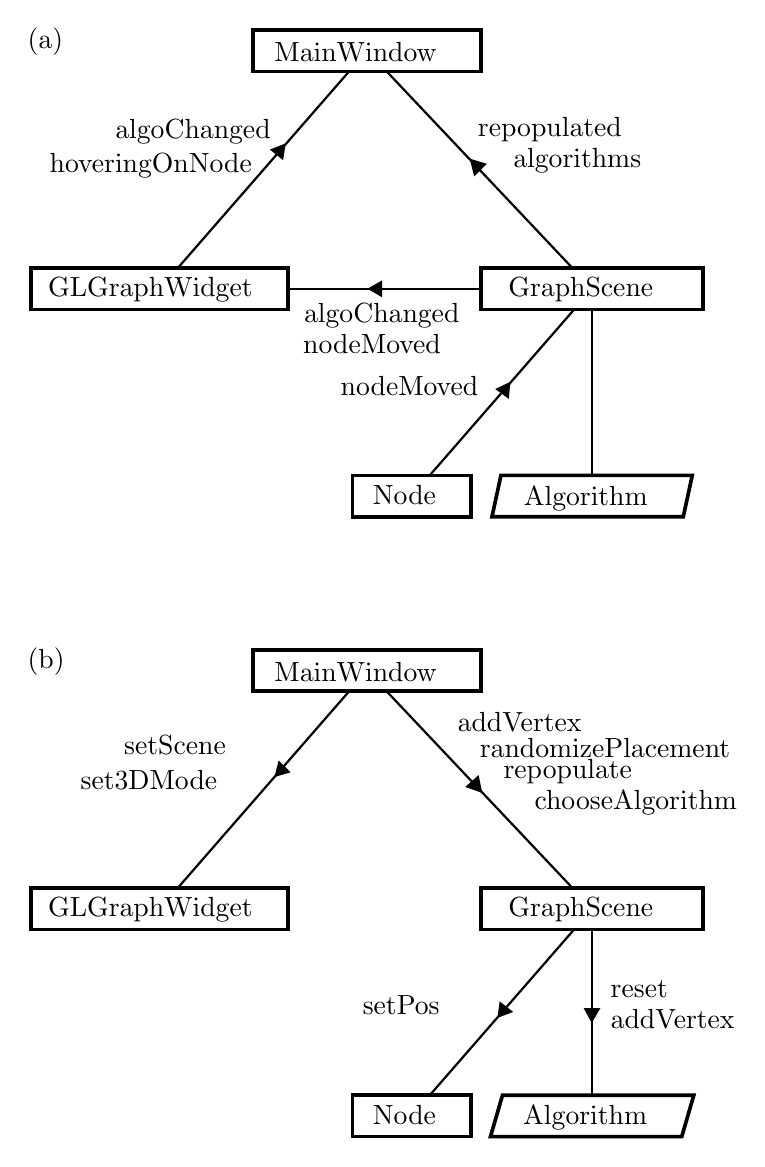
\begin{tikzpicture}[y=0.80pt, x=0.8pt,yscale=-1, inner sep=0pt, outer sep=0pt]
\begin{scope}[shift={(-112.55702,-213.37695)}]
  \begin{scope}[cm={{0.60244614,0.0,0.0,0.60244614,(61.856524,54.195329)}}]
    \path[draw=black,line width=1.328pt,rounded corners=0.0000cm]
      (268.2596,281.6544) rectangle (438.9601,312.6544);
    \path[fill=black] (284.14697,305.60364) node[above right] (text3003) {MainWindow
      };
  \end{scope}
  \begin{scope}[cm={{0.60244614,0.0,0.0,0.60244614,(41.49929,104.70602)}}]
    \path[fill=black] (148.19138,401.63339) node[above right] (text2991)
      {GLGraphWidget       };
    \path[draw=black,line width=1.328pt,rounded corners=0.0000cm]
      (135.3776,376.3655) rectangle (328.3015,407.3655);
  \end{scope}
  \begin{scope}[cm={{0.60244614,0.0,0.0,0.60244614,(88.967165,105.34863)}}]
    \path[fill=black] (414.52719,400.70734) node[above right] (text2995) {GraphScene
      };
    \path[draw=black,line width=1.328pt,rounded corners=0.0000cm]
      (393.9723,375.2989) rectangle (560.6322,406.2989);
  \end{scope}
  \begin{scope}[cm={{0.60244614,0.0,-0.13122252,0.60244614,(154.0838,136.35127)}}]
    \path[fill=black] (428.1041,505.48331) node[above right] (text2987) {Algorithm
      };
    \path[draw=black,line width=1.328pt,rounded corners=0.0000cm]
      (405.2505,479.1763) rectangle (548.6769,510.1763);
  \end{scope}
  \path[draw=black,line join=miter,line cap=butt,line width=0.800pt]
    (189.3056,331.4460) -- (266.7520,242.5528);
  \path[draw=black,line join=miter,line cap=butt,line width=0.800pt]
    (283.7097,242.5528) -- (367.6938,331.4460);
  \path[draw=black,line join=miter,line cap=butt,line width=0.800pt]
    (326.3143,340.7839) -- (239.2832,340.7839);
  \path[draw=black,line join=miter,line cap=butt,line width=0.800pt]
    (376.5161,350.1218) -- (376.5161,425.0292);
  \path[fill=black] (246.43787,358.36713) node[above right] (text3059)
    {algoChanged     };
  \path[fill=black] (246.03421,370.05441) node[above right] (text3063) {nodeMoved
    };
  \path[cm={{0.60244614,0.0,0.0,0.60244614,(219.19954,185.07318)}},draw=black,fill=black,line
    join=miter,line cap=butt,miter limit=4.00,line width=1.328pt]
    (102.3179,254.4263) -- (102.2747,262.3632) -- (95.4227,258.3573) -- cycle;
  \path[cm={{0.59608163,0.08733863,-0.08733863,0.59608163,(198.29375,115.77633)}},draw=black,fill=black,line
    join=miter,line cap=butt,miter limit=4.00,line width=1.328pt]
    (102.3179,254.4263) -- (102.2747,262.3632) -- (95.4227,258.3573) -- cycle;
  \path[cm={{-0.69799145,0.17382972,-0.18444507,-0.71573379,(441.95326,452.94883)}},draw=black,fill=black,line
    join=miter,line cap=butt,miter limit=4.00,line width=1.097pt]
    (102.3179,254.4263) -- (102.2747,262.3632) -- (95.4227,258.3573) -- cycle;
  \path[fill=black] (161.1712,275.12494) node[above right] (text3118) {algoChanged
    };
  \path[fill=black] (131.48926,290.81223) node[above right] (text3122)
    {hoveringOnNode     };
  \begin{scope}[cm={{0.60244614,0.0,0.0,0.60244614,(80.129239,88.883392)}}]
    \path[fill=black] (327.60049,579.53265) node[above right] (text3128) {Node
      };
    \path[draw=black,line width=1.328pt,rounded corners=0.0000cm]
      (312.2591,557.9682) rectangle (401.1372,588.9682);
  \end{scope}
  \path[draw=black,line join=miter,line cap=butt,line width=0.800pt]
    (303.1524,425.0292) -- (368.3843,350.1218);
  \path[cm={{0.58190708,0.05230551,-0.04887953,0.5983474,(291.49485,226.59278)}},draw=black,fill=black,line
    join=miter,line cap=butt,miter limit=4.00,line width=1.351pt]
    (102.3179,254.4263) -- (102.2747,262.3632) -- (95.4227,258.3573) -- cycle;
  \path[fill=black] (262.92914,388.73416) node[above right] (text3146) {nodeMoved
    };
  \path[fill=black] (324.94656,274.44034) node[above right] (text3150)
    {repopulated     };
  \path[fill=black] (121.5652,235.30273) node[above right] (text3889) {(a)     };
  \begin{scope}[cm={{0.60244614,0.0,0.0,0.60244614,(61.856524,334.19533)}}]
    \path[draw=black,line width=1.328pt,rounded corners=0.0000cm]
      (268.2596,281.6544) rectangle (438.9601,312.6544);
    \path[fill=black] (284.14697,305.60364) node[above right] (text3901) {MainWindow
      };
  \end{scope}
  \begin{scope}[cm={{0.60244614,0.0,0.0,0.60244614,(41.49929,384.70602)}}]
    \path[fill=black] (148.19138,401.63339) node[above right] (text3907)
      {GLGraphWidget       };
    \path[draw=black,line width=1.328pt,rounded corners=0.0000cm]
      (135.3776,376.3655) rectangle (328.3015,407.3655);
  \end{scope}
  \begin{scope}[cm={{0.60244614,0.0,0.0,0.60244614,(88.967165,385.34863)}}]
    \path[fill=black] (414.52719,400.70734) node[above right] (text3915) {GraphScene
      };
    \path[draw=black,line width=1.328pt,rounded corners=0.0000cm]
      (393.9723,375.2989) rectangle (560.6322,406.2989);
  \end{scope}
  \begin{scope}[cm={{0.60244614,0.0,-0.17496336,0.60244614,(175.72135,416.35127)}}]
    \path[fill=black] (428.44839,505.48331) node[above right] (text3923) {Algorithm
      };
    \path[draw=black,line width=1.328pt,rounded corners=0.0000cm]
      (405.2505,479.1763) rectangle (548.6769,510.1763);
  \end{scope}
  \path[draw=black,line join=miter,line cap=butt,line width=0.800pt]
    (189.3056,611.4460) -- (266.7520,522.5528);
  \path[draw=black,line join=miter,line cap=butt,line width=0.800pt]
    (283.7097,522.5528) -- (367.6938,611.4460);
  \path[draw=black,line join=miter,line cap=butt,line width=0.800pt]
    (376.5161,630.1218) -- (376.5161,705.0292);
  \path[cm={{-0.58532849,-0.14258998,0.14258998,-0.58532849,(257.79281,723.57069)}},draw=black,fill=black,line
    join=miter,line cap=butt,miter limit=4.00,line width=1.328pt]
    (102.3179,254.4263) -- (102.2747,262.3632) -- (95.4227,258.3573) -- cycle;
  \path[cm={{0.70569892,-0.13927625,0.14900577,0.72394207,(214.68757,391.73552)}},draw=black,fill=black,line
    join=miter,line cap=butt,miter limit=4.00,line width=1.097pt]
    (102.3179,254.4263) -- (102.2747,262.3632) -- (95.4227,258.3573) -- cycle;
  \path[fill=black] (165.1712,551.12494) node[above right] (text3951) {setScene
    };
  \path[fill=black] (145.48926,566.81226) node[above right] (text3955) {set3DMode
    };
  \begin{scope}[cm={{0.60244614,0.0,0.0,0.60244614,(80.129239,368.88339)}}]
    \path[fill=black] (327.60049,579.53265) node[above right] (text3961) {Node
      };
    \path[draw=black,line width=1.328pt,rounded corners=0.0000cm]
      (312.2591,557.9682) rectangle (401.1372,588.9682);
  \end{scope}
  \path[draw=black,line join=miter,line cap=butt,line width=0.800pt]
    (303.1524,705.0292) -- (368.3843,630.1218);
  \path[cm={{0.35985131,-0.46028117,0.47594756,0.3658999,(177.46665,618.17186)}},draw=black,fill=black,line
    join=miter,line cap=butt,miter limit=4.00,line width=1.351pt]
    (102.3179,254.4263) -- (102.2747,262.3632) -- (95.4227,258.3573) -- cycle;
  \path[fill=black] (272.92914,668.73413) node[above right] (text3971) {setPos
    };
  \path[fill=black] (315.80371,540.58319) node[above right] (text3975) {addVertex
    };
  \path[fill=black] (121.5652,515.30273) node[above right] (text3979) {(b)     };
  \path[fill=black] (325.80371,552.58319) node[above right] (text3983)
    {randomizePlacement     };
  \path[fill=black] (336.51801,564.58319) node[above right] (text3987) {repopulate
    };
  \path[fill=black] (340.94656,288.44034) node[above right] (text3991) {algorithms
    };
  \path[fill=black] (350.51801,578.58319) node[above right] (text3995)
    {chooseAlgorithm     };
  \path[cm={{0.50323671,0.29682408,-0.30078027,0.51955755,(403.81881,503.95313)}},draw=black,fill=black,line
    join=miter,line cap=butt,miter limit=4.00,line width=1.351pt]
    (102.3179,254.4263) -- (102.2747,262.3632) -- (95.4227,258.3573) -- cycle;
  \path[fill=black] (384.92914,660.73413) node[above right] (text4001) {reset
    };
  \path[fill=black] (384.92914,674.73413) node[above right] (text4005) {addVertex
    };
\end{scope}

\end{tikzpicture}

  \caption{Flow of (a) information upwards via \code{signal}s and (b)
    commands downward}
  \label{fig:interaction}
\end{figure}

\subsection{Graph drawing}

We looked into various graphics libraries which allow for
platform-independent drawing using primitives. Candidates were
\buzz{Cairo}\footnote{Cairo homepage: http://cairographics.org/},
\buzz{Qt} and \buzz{OpenGL}. The first two are the
most common 2D drawing libraries used in modern open-source
software; however, as they operate solely on the CPU, they proved
too slow for the large graphs we wished to visualise.

Therefore we decided to use \buzz{OpenGL} for drawing graphs on
the screen. Thanks to its hardware accelerated nature, we can now
(re-)draw thousands of nodes and edges often enough every second
to give the user the impression of a smooth interface when interacting
with the graph.

Implementing the camera handling, the node/edge drawing and the
interface allowing the user to `fly' through a 3D graph we also
developed a helper library, \code{glAncillary}. A significant portion
of our code can now be reused in similar projects using OpenGL,
and this is important since applications such as Visigoth require a
completely different type of graphics engine compared to the ones
commonly found e.g. in video games.


\subsection{Graph layout}
Laying out a graph is a tricky problem, mainly due to the fact that the
prime interest when engineering layouts is to please humans' taste
instead of some logical property. A wide array of such algorithms have
been proposed, and since drawing graphs is a central task in Visigoth,
we had to choose the one that fit best.

First we experimented with the existing solutions. One of the most
complete free graph-drawing algorithm is
OpenViz\footnote{\url{http://www.graphviz.org/}}, and it provides
various algorithms:

\begin{description}
\item [dot] A hierarchical layout, used for directed graphs. Our small
  world networks are not directed and it was clear from the beginning
  that they did not fit this model well.

\item [twopi, circo] Radial and circular layout, respectively. Again,
  unsuitable for the quasi-random networks that we use in Visigoth.

\item [neato] A spring model layout, which seemed to work reasonably
  well with random graphs.
\end{description}

The spring model seemed to be the best fit. This class of algorithm
work by treating edges like springs: in this way clusters of highly
connected nodes would be drawn together. To counter this force (that
would lead to nodes lumping together), nodes are treated as charged
particles of the same polarity, causing repulsion between every node
and the others.

When generating a graph, the nodes are first places at random
locations in the space. Then, we apply the algorithm repeatedly until
the forces are low enough that we can consider the graph to be stable.

Spring model algorithms are nice for two reasons:

\begin{itemize}
\item Good results: spring force algorithms produce pleasant graphs
  for almost all kind of networks. Some algorithms might produce
  better results for specific kinds of graph, but spring force
  algorithms are by far the more adaptive.

\item Ease of implementation: Our simple implementation of the
  algorithm take a little less then 50 lines of C++ code, and works
  well up to medium-sized graphs.

\item Real time drawing: force based algorithms can be used to show in
  real time the untangling of the graph, which is usually an
  interesting effect. It also permits interaction, for example in the
  form of node-dragging that changes the shape of the graph. We employ
  both techniques in Visigoth.
\end{itemize}

\subsubsection{FADE}

However, even a simple description of the algorithms reveals its high
cost. For each particle, we need to iterate through all the connected
nodes to calculate the spring forces, and more importantly through all
the particles of the graphs to calculate the repulsion forces. Thus,
the algorithm is \(O(n^2)\), where \(n\) is the number of nodes.

For this reason, our implementation works smoothly up to around a
\(1000\) nodes, but then performance degrades quickly, and the program
becomes unresponsive. Various solutions have been studied, most of
which rely on various approximations.

We chose to implement the \emph{FADE} algorithm \cite{fade}, which works by
recursively subdividing the graph space into sub-spaces, and then
treats sub-spaces as single particles when they are far enough. This
algorithm, while improving performance, is a lot more complex then the
naive one.

\begin{figure}
  \centering
  \subfloat[Graph view]{
    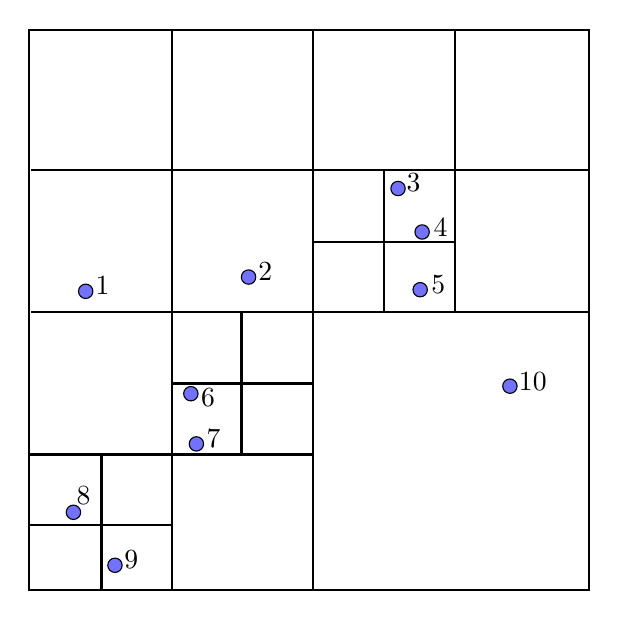
\begin{tikzpicture}[y=0.80pt, x=0.8pt,yscale=-0.5, xscale=0.5, inner sep=0pt, outer sep=0pt]
  \path[draw=black,line join=miter,line cap=butt,line width=0.800pt]
  (356.4286,94.5050) -- (356.4286,598.7908);
  \path[draw=black,line join=miter,line cap=butt,line width=0.800pt]
  (102.1429,348.7908) -- (605.7143,348.7908);
  \path[draw=black,line join=miter,line cap=butt,line width=0.800pt]
  (102.1429,220.2193) -- (607.1429,220.2193);
  \path[draw=black,line join=miter,line cap=butt,line width=0.800pt]
  (229.2857,93.0765) -- (229.2857,598.7908);
  \path[draw=black,line join=miter,line cap=butt,line width=0.800pt]
  (485.0000,93.7908) -- (485.0000,349.5050);
  \path[draw=black,line join=miter,line cap=butt,line width=0.800pt]
  (101.4286,477.3622) -- (356.4286,477.3622);
  \path[draw=black,line join=miter,line cap=butt,line width=0.800pt]
  (420.7143,220.2193) -- (420.7143,349.5050);
  \path[draw=black,line join=miter,line cap=butt,line width=0.800pt]
  (356.4286,285.2193) -- (485.0000,285.2193);
  \path[draw=black,line join=miter,line cap=butt,line width=0.800pt]
  (292.1429,348.0765) -- (292.1429,476.6479);
  \path[draw=black,line join=miter,line cap=butt,line width=0.800pt]
  (228.5714,413.0765) -- (357.1429,413.0765);
  \path[draw=black,line join=miter,line cap=butt,line width=0.800pt]
  (165.7143,477.3622) -- (165.7143,599.5050);
  \path[draw=black,line join=miter,line cap=butt,line width=0.800pt]
  (100.7143,540.9336) -- (229.2857,540.9336);
  \path[cm={{0.86607143,0.0,0.0,0.86607143,(-133.53636,-75.700851)}},draw=black,fill=c7372ff]
  (506.4286,453.4336)arc(0.000:180.000:7.500)arc(-180.000:0.000:7.500) -- cycle;
  \path[cm={{0.86607143,0.0,0.0,0.86607143,(-280.6792,-62.843726)}},draw=black,fill=c7372ff]
  (506.4286,453.4336)arc(0.000:180.000:7.500)arc(-180.000:0.000:7.500) -- cycle;
  \path[cm={{0.86607143,0.0,0.0,0.86607143,(-185.6792,29.656274)}},draw=black,fill=c7372ff]
  (506.4286,453.4336)arc(0.000:180.000:7.500)arc(-180.000:0.000:7.500) -- cycle;
  \path[cm={{0.86607143,0.0,0.0,0.86607143,(-180.6792,75.013418)}},draw=black,fill=c7372ff]
  (506.4286,453.4336)arc(0.000:180.000:7.500)arc(-180.000:0.000:7.500) -- cycle;
  \path[cm={{0.86607143,0.0,0.0,0.86607143,(-291.75062,136.79913)}},draw=black,fill=c7372ff]
  (506.4286,453.4336)arc(0.000:180.000:7.500)arc(-180.000:0.000:7.500) -- cycle;
  \path[cm={{0.86607143,0.0,0.0,0.86607143,(-254.25063,184.65628)}},draw=black,fill=c7372ff]
  (506.4286,453.4336)arc(0.000:180.000:7.500)arc(-180.000:0.000:7.500) -- cycle;
  \path[cm={{0.86607143,0.0,0.0,0.86607143,(102.53509,22.87056)}},draw=black,fill=c7372ff]
  (506.4286,453.4336)arc(0.000:180.000:7.500)arc(-180.000:0.000:7.500) -- cycle;
  \path[cm={{0.86607143,0.0,0.0,0.86607143,(21.463659,-64.272297)}},draw=black,fill=c7372ff]
  (506.4286,453.4336)arc(0.000:180.000:7.500)arc(-180.000:0.000:7.500) -- cycle;
  \path[cm={{0.86607143,0.0,0.0,0.86607143,(23.249374,-116.41515)}},draw=black,fill=c7372ff]
  (506.4286,453.4336)arc(0.000:180.000:7.500)arc(-180.000:0.000:7.500) -- cycle;
  \path[cm={{0.86607143,0.0,0.0,0.86607143,(1.4636592,-155.70087)}},draw=black,fill=c7372ff]
  (506.4286,453.4336)arc(0.000:180.000:7.500)arc(-180.000:0.000:7.500) -- cycle;
  \path[fill=black] (160.31509,332.78058) node[above right] (text6462) {1};
  \path[fill=black] (307.43341,319.70856) node[above right] (text6462-4) {2};
  \path[fill=black] (441.40405,239.94313) node[above right] (text6462-9) {3};
  \path[fill=black] (465.61832,280.30029) node[above right] (text6462-98) {4};
  \path[fill=black] (463.73944,332.14725) node[above right] (text6462-5) {5};
  \path[fill=black] (255.68974,433.98373) node[above right] (text6462-0) {6};
  \path[fill=black] (260.68976,470.65741) node[above right] (text6462-7) {7};
  \path[fill=black] (143.21951,522.34161) node[above right] (text6462-3) {8};
  \path[fill=black] (186.40405,580.65741) node[above right] (text6462-43) {9};
  \path[fill=black] (542.83264,419.586) node[above right] (text6462-02) {10};
  \path[draw=black,line join=miter,line cap=butt,line width=0.800pt]
  (606.0915,92.7173) -- (606.0915,599.8138) -- (100.0051,599.8138) --
  (100.0051,92.7173);
  \path[draw=black,line join=miter,line cap=butt,line width=0.800pt]
  (100.0051,93.7274) -- (605.0814,93.7274);
\end{tikzpicture}

  }
  \hspace{10pt}
  \subfloat[Tree representation]{
    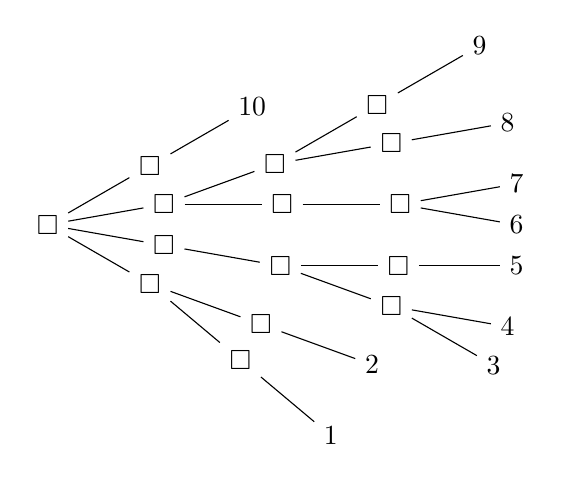
\begin{tikzpicture}[grow cyclic]
  \node {\square}
  child {
    node {\square}
    child {
      node {\square}
      child {node {1}}
    }
    child {
      node {\square}
      child {node {2}}
    }
  }
  child {
    node {\square}
    child {
      node {\square}
      child {
        node {\square}
        child { node{3} }
        child { node{4} }
      }
      child {
        node {\square}
        child {node{5}}
      }
    }
  }
  child {
    node {\square}
    child {
      node {\square}
      child {
        node {\square}
        child {node{6}}
        child {node{7}}
      }
    }
    child {
      node {\square}
      child {
        node {\square}
        child {node{8}}
      }
      child {
        node {\square}
        child {node{9}}
      }
    }
  }
  child {
    node {\square}
    child { node {10} }
  }
  ;
\end{tikzpicture}

  }
  \caption{The QuadTree for a sample graph, empty branches omitted}
  \label{fig:quadtree}
\end{figure}

The first step is to build a data structure representing the recursive
subdivision. This kind of data structure is called a \emph{TreeCode},
which recursively subdivides the space until only one node remains in
the current space, or a maximum depth/minimum space size size is
hit. The space decomposition can be irregular (e.g. \emph{Voronoi}
spaces) or regular. In the latter case, the space is recursively
subdivided in squares. We chose to use a regular, 4-way space
decomposition, mainly due to its simplicity. This kind of structure is
called \emph{QuadTree}. Figure \ref{fig:quadtree} shows a sample
QuadTree for a Visigoth graph. In the QuadTree, each sub-quadrant
preserved the weighted centre of gravity relative to the contained
nodes.

Building the tree is the difficult part of the algorithm and can be
done in linear time. Once that is done, to calculate the non-edge
forces for a given node the algorithm proceeds as indicated in figure
\ref{proc:FADE}.

\begin{figure}[ht]
  \begin{minipage}[b]{0.5\linewidth}
    \begin{algorithmic}
  \REQUIRE \(0 < \theta < 1\)
  \REQUIRE \(\beta > 1\)
  \REQUIRE \(\vec{n} \neq \vec{q}\)
\end{algorithmic}
force\((n, q)\):
\begin{algorithmic}
  \STATE \(\vec{d} \gets \vec{n} - \vec{q}\)
  \IF { \(q\) is terminal \OR \(\frac{\vec{d}}{\textrm{width}(q)} < \theta\) }
  \STATE \(\vec{v} \gets \vec{d} \cdot \frac{\beta}{|{\vec{d}}|^2}\)
  \STATE \(\vec{v} \gets \vec{v} \cdot \textrm{mass}(q)\)
  \RETURN \(\vec{v} \cdot \frac{\beta}{|{\vec{d}}|^2}\)
  \ELSE
  \STATE \(\vec{v} \gets 0\)
  \FOR {\(q'\) in children\((q)\)}
  \STATE \(\vec{v} \gets \vec{v} + \textrm{force}(n, q')\)
  \ENDFOR
  \RETURN \(\vec{v}\)
  \ENDIF
\end{algorithmic}

    \caption{This procedure calculates the non-edge force of a given
      node \(n\), given the QuadTree \(q\). \(\vec{n}\) and
      \(\vec{q}\) indicate the vectors corresponding to the respective
      centers of gravity. \(\beta\) is an empirically determined
      parameter used to regulate the amount of force - \(75\) has
      worked well for us. \(\theta\) is central to the FADE algorithm
      and determines the amount of approximation. If \(\geq 1\) the
      algorithm is unstable, we used values between \(0.5\) and
      \(0.8\). See figure \ref{fig:theta} for a visual
      explanation. The mass of a quadrant is simply the number of
      nodes residing in it. }
    \label{proc:FADE}
  \end{minipage}
  \hspace{10pt}
  \begin{minipage}[b]{0.5\linewidth}
    \centering
    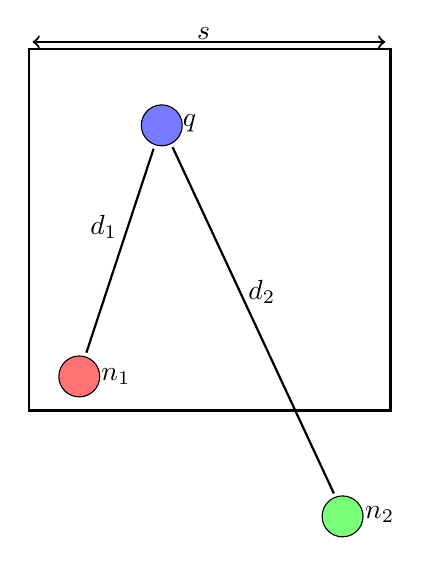
\begin{tikzpicture}[y=0.80pt, x=0.8pt,yscale=-1, inner sep=0pt, outer sep=0pt]
  \path[draw=black,fill=cffffff,line join=miter,line cap=butt,fill
    opacity=0.000,even odd rule,line width=0.803pt,rounded corners=0.0000cm]
  (140.4134,176.5621) rectangle (303.7579,339.9066);
  \path[cm={{0.79503474,0.0,0.0,0.79503474,(-296.23722,-12.403676)}},draw=black,fill=c787aff]
  (636.3961,281.1107)arc(0.000:180.000:11.617)arc(-180.000:0.000:11.617) --
  cycle;
  \path[cm={{0.79503474,0.0,0.0,0.79503474,(-333.50701,101.01225)}},draw=black,fill=cff7374]
  (636.3961,281.1107)arc(0.000:180.000:11.617)arc(-180.000:0.000:11.617) --
  cycle;
  \path[cm={{0.79503474,0.0,0.0,0.79503474,(-214.57843,164.22654)}},draw=black,fill=c79ff79]
  (636.3961,281.1107)arc(0.000:180.000:11.617)arc(-180.000:0.000:11.617) --
  cycle;
  \path[draw=black,line join=miter,line cap=butt,line width=0.800pt]
  (166.4286,313.7908) -- (196.7857,221.6479);
  \path[draw=black,line join=miter,line cap=butt,line width=0.800pt]
  (205.3571,220.9336) -- (278.2143,377.3622);
  \path[fill=black] (168.21428,262.36218) node[above right] (text5235) {\(d_1\)};
  \path[fill=black] (239.64287,291.64789) node[above right] (text5239) {\(d_2\)};
  \path[fill=black] (216.42857,172.36218) node[above right] (text5243) {\(s\)};
  \path (142.5000,173.7908) -- (300.0000,173.7908);
  \path[draw=black,line join=miter,line cap=butt,line width=0.800pt, <->]
  (142.1429,173.4336) -- (301.4286,173.4336);
  \path[fill=black] (210,214.1479) node[above right] (text5479) {\(q\)};
  \path[fill=black] (173.21429,328.07648) node[above right] (text5483) {\(n_1\)};
  \path[fill=black] (292.34625,390.3728) node[above right] (text5483-5) {\(n_2\)};
\end{tikzpicture}

    \caption{In this case, \(n_1\) and \(n_2\) are nodes and \(q\) is
      a quadrant with edge length \(s\). When calculating the non-edge
      force between \(n_1\) and \(q\), where \(s\) is the quadrant
      will be judged to be too close to approximate, since
      \(\frac{s}{d_1} > 1\), while \(n_2\) might be judged far enough,
      depending on \(\theta\).}
    \label{fig:theta}
  \end{minipage}
\end{figure}

Once implemented, the FADE algorithm lead to great speedups while
preserving good node placements. While drawing \(1000\) nodes is
already difficult with the simple algorithm, FADE can easily handle
\(10000\) nodes, after which other performance limits are hit (the
graph generation time and the OpenGL drawing).

After we implemented the 3D view we had to write an extension to FADE to support
3D, which proved to be straight forward. Now we have a 3-dimensional space,
which is recursively divided into $8$ cubes.

\subsection{Effort}

Work was divided between team members such that each would focus on
developing a particular component and reviewing another. Table
\ref{fig:effort} gives an overview of the distribution of work and the
amount of effort required to finish each component.

\begin{figure}[h]
  \centering
  \begin{tabular}{c|c|c}
    Component         & Team members    & Effort \\
    \hline
    GUI               & Ingrid, Max     & ~80 phrs \\
    3D Renderer       & Max, Francesco  & ~60 phrs\\
    \code{GraphScene} & Francesco, Alex & ~80 phrs\\
    Algorithms        & Marc, Ingrid    & ~120 phrs\\
    Testing           & Alex, Marc      & ~20 phrs\\
    \hline
    Total             &                 & ~360 phrs
  \end{tabular}
  \caption{Effort expanded on each component in person-hours}
  \label{fig:effort}
\end{figure}

An \emph{impact} graph, as generated by
Github \footnote{\url{https://github.com}} is included in Figure
\ref{fig:impact}. It shows that, at least in terms of
SLOC \footnote{\url{http://en.wikipedia.org/wiki/Source_lines_of_code}},
the effort was well spread out across the development team.

\begin{figure}[h]
  \centering
  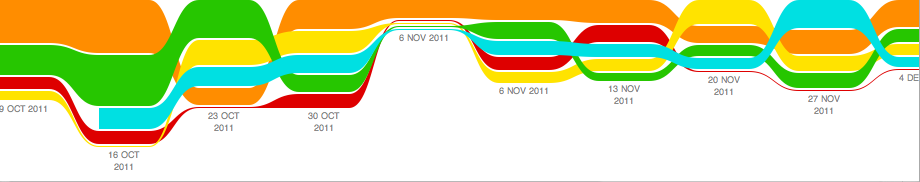
\includegraphics[width=\textwidth]{impact.png}
  \caption{Development impact of team members}
  \label{fig:impact}
\end{figure}

The total amount of code\footnote{as generated using David
  A. Wheeler's `SLOCCount'} required for each component is included in
Figure \ref{fig:sloc}. Note that this table does not show the all the
code that did \emph{not} make it into the final product; for instance,
the renderer went through two complete rewrites before being the
current 3D Renderer.

\begin{figure}[h]
  \centering
  \begin{tabular}{c|l}
    Component         & SLOC \\
    \hline
    GUI               & $180$ C++, 1037 XML\\
    3D Renderer       & $452$ C++, 82 C\\
    \code{GraphScene} & $686$ C++\\
    Algorithms        & $1220$ C++\\
    Testing           & $238$ C++ \\
    \hline
    Total             & $3061$ C++, $1037$ XML, $82$ C
  \end{tabular}
  \caption{Lines of code in each component}
  \label{fig:sloc}
\end{figure}

\subsection{Development methodologies}
% FIXME: This is text from Report 3.

\subsubsection{Peer review}
Our rule of thumb, ``\emph{the master branch is always releasable}'',
has been
the foundation of our testing practices. To adhere to this, we have
had to ensure that no bugs crept into the master branch. Towards this
goal, no changes are merged into master until at least another member
of the team reviews them. Through this practice of peer review the
whole team has stayed informed on the current state of the project
in addition to exposing and fixing bugs missed by the original code
author. While this does indeed slow done writing code, we like to
think that it otherwise shortens overall development time.

\subsubsection{Scrum}
To further promote group awareness of the complete state of the
project we held frequent short meetings true to the idea of scrum.
These were whole-group meetings held every few days, in which team
members shared comments on what features they were working on at
the time and the future outlook of the project.

\subsubsection{Client feedback}
Towards the end of each iteration, we held meetings with our client
in order to report on our progress and get feedback on new
developments. These meetings would consist of a short demo of newly
added features, a short "impromptu" usability test and a discussion
on what new features should be the focus of the following iteration.

The feedback we received at the end of each iteration was
consistently positive. The Visigoth interface always met our
client's demands and only minor changes have been made from
iteration to iteration, e.g. button placements. Most of the our
client's wishes referred to extensions to the functionality of
our product, such as a 3D rendering mode and the network generation
algorithms.


\subsubsection{Other users' feedback}
Near the end of each iteration we asked classmates and friends for
their sincere point of view concerning our progress and project
overall, to that specific point in time.

The last impression was that they were mainly happy. We followed their
advice when it appeared. For example, at some point, they wanted to be
able to customize the graph a bit more following their own taste. So,
we added the possibility to change the color of the nodes, edges,
background; to highlight selected nodes as well as their direct
neighbours.



\section{Looking back}
%% This section corresponds to 'Conclusions' in part D of the requirements

\subsection{Validation}
%% The client is a happy puppy
% FIXME: This is text from Report 3

\subsubsection{Tests}
To automate regression detection we use a test suite written using
the Qt Unit-Testing framework, which covers a significant portion
of the codebase. In particular, it completely covers the intricate
algorithmic and UI logic encoded in the Algorithm classes. Running
the test suite can expose changes breaking rarely-used functions
which would have slipped past a quick tests by the coder.

The tests we use to determine our product's integrity are split
into two categories: system and interface tests. System tests focus
on the Visigoth back-end, i.e. memory consistency and build stability.
The interface tests were deployed to ensure that user input in the
graphical interface is successfully passed to and feedback returned
from the system's back-end. More specifically, the interface tests
encode a number of common use-cases and ensure that Visigoth indeed
behaves as per the user's expectations.

These user interface tests proved quite useful and revealed several
problems, all of them caused by internal API changes and code not
being updated to reflect the changes. These would manifest as
misleading readings on the Visigoth graph-information panels and
were thus caught by the use-case tests.

When testing our product, the most profound fault that was revealed
by our system tests were memory leaks, found in two separate
instances. The lessons to take away were twofold:
\begin{itemize}
  \item One the one hand, old code that sees no use and just rots
        should be removed immediately so that it cannot interfere
        with the newer infrastructure. We were still semi-maintaining
        internal structures for an old rendering front-end, though
        not cleaning them up properly. We have recently began to
        track test coverage statistics. These should help us in
        identifying dead and duplicate code in the future.
  \item On the other hand, even a three-way merges as done by Git
        should be done with great care: merge conflicts between
        diverged branches may re-introduce old code, leading to
        the situation described above.
\end{itemize}

\subsubsection{Continuous Integration}
We use a Jenkins CI\footnote{http://jenkins-ci.org/} server. It is
set up to track the master branch. On receiving a change notification
from the central repository, it proceeds to do a fresh build of the
project, runs the tests and generates the coverage statistics. It
also keeps track of previous builds and aggregates information about
the overall health of the project.
The server is publicly accessible so that interested parties can get
a rough idea of what the current status of the project is. It is also
set up to notify team members (via the project mailing-list) when
problems occur.

\subsubsection{Stability under load}
Load-testing Visigoth is a straightforward affair: generate networks
with a large number of nodes. We have found our software to stay
sufficiently responsive even under load. This is especially true
since it is usually generating a high CPU load itself when
recalculating the node positions using the spring force model. In
particular, we met our initial goal of displaying thousands of nodes
in real-time.

\subsubsection{Style}
We have strived to use consistent style throughout the code and
documentation. To this extent, it fell to the reviewer doing the
merge to mention and fix any style issues. This has worked adequately
most of the time, and in the few instances where badly styled code
slipped through, subsequent global reviews remedied the problem in a
timely fashion.


\subsection{Documentation}
% FIXME: This is text from Report 3.

\subsubsection{Tools and policies}
We use Git\footnote{http://git-scm.com/} to manage our code base and
to enable parallel development; using its lightweight branching
extensively in our work-flow. Additionally, the distributed nature
of Git enabled more efficient peer reviews, as we could pull/push
changes directly from one another. As a general policy, code needed
to be checked and corrected by at least one other developer before it
made its way into the master branch.

\subsubsection{Knowledge transfer}
Due to our peer review scheme, at least two people would know every
bit of code. Also, mutual interest in each other's area of expertise
has fostered cooperation in labs where problems were solved together
in eXtreme Programming setups (one person coding, the other watching
and correcting).

We also held periodic "Direct Mental Download" meetings in which one
team-member would dump his accumulated knowledge into the willing
minds of other team-member (referred to as recipients in our terminology).

Additionally, we shared relevant articles/papers between us to ease
the used principles understanding and to improve the existent work.
This exchange of written or verbal knowledge transfer allowed us not
only to improve team-working but to gain new technical skills as well.

%Add the Log-Book in appendix


\subsection{Functional testing}
\label{tests}




\subsection{People management and contributions}
%This is from Report 2 except the summary of contributions which is a new add

\subsection{Lessons learned}


\subsection{Ethical and Environmental Impact}
%Check Report 2

\addcontentsline{toc}{section}{References}
\begin{thebibliography}{9}

\bibitem{hamm10}
  David A. Hammond,
  \emph{Altruism in Small World Models}.
  Imperial College London,
  2010.

\bibitem{oconn11}
  Luke M. O'Connor,
  \emph{Algorithms for Constructing Realistic Networks}.
  Imperial College London,
  2011.

\bibitem{fade}
  Aaron Quigley and Peter Eades,
  \emph{FADE: Graph drawing, clustering and visual abstraction}.
  Department of Computer Science and Software Engineering,
  Univ. of  Newcastle, Australia, 2000.

\bibitem{complexAdapt}
Claudius Gros,
\emph{Complex and Adaptive Dynamical Systems}.
Springer,
2008.

\bibitem{complexNets}
  \url{http://en.wikipedia.org/wiki/Complex_network}

\end{thebibliography}

\end{document}
